\documentclass[12pt,a4paper,twoside]{book}
\usepackage{pgfgantt}

\usepackage[hang, flushmargin]{footmisc}         %Problem line.
\PassOptionsToPackage{hyphens}{url}\usepackage[hyperfootnotes=false]{hyperref}
\usepackage{footnotebackref}

\usepackage{tikz}
\usetikzlibrary{shapes,arrows}	
\usepackage{graphicx}
\usepackage{wrapfig}
\usepackage{lipsum}
\usepackage{float}
\usepackage{caption}
\usepackage{subcaption}
\usepackage[nameinlink]{cleveref}
\usepackage{notoccite}
\usepackage{amsmath}
\usepackage{listings}


\makeatletter
\renewcommand\footnoterule{%
  \kern6\p@
  \hrule\@width \textwidth
  \kern2.6\p@}
\makeatother

\setcounter{secnumdepth}{3} 
\setcounter{tocdepth}{3}
% only chapter and sections will be numbered
%\setcounter{secnumdepth}{3} % default value for 'report' class is "2"


%\floatstyle{boxed} 
\restylefloat{figure}


\setlength{\textfloatsep}{5pt plus 1.0pt minus 2.0pt}

%include the configuration file for layout
%Have a look in this file it has some useful commands defined
\usepackage{setspace}
\usepackage{geometry}
\usepackage[toc,page]{appendix}
\usepackage{lipsum}
\usepackage[export]{adjustbox}
\usepackage[T1]{fontenc}
\usepackage{textcomp}
\usepackage{epsfig,graphics}
\usepackage{graphicx}
\usepackage{titlesec}


%%%%%%%%%%%%%%%%%%%%%%%%%%%%%%%%%%%%%%%%%%%%%%%%%%%%%%%%%%%%%%%%%%%%%%%%%%%%%%
% Details of your dissertation
%%%%%%%%%%%%%%%%%%%%%%%%%%%%%%%%%%%%%%%%%%%%%%%%%%%%%%%%%%%%%%%%%%%%%%%%%%%%%%
\newcommand{\projectTitle}{The Robot Shopkeeper: An Integrated System for Robotic Manipulation and Perception}
\newcommand{\fullname}{Kieran Marshall Haden}
\newcommand{\degreeTitle}{BSc Artificial Intelligence}
\newcommand{\session}{Session 2015/2016}

%%%%%%%%%%%%%%%%%%%%%%%%%%%%%%%%%%%%%%%%%%%%%%%%%%%%%%%%%%%%%%%%%%%%%%%%%%%%%%
% Change the geometry of the page to have a 25 mm binding edge
%%%%%%%%%%%%%%%%%%%%%%%%%%%%%%%%%%%%%%%%%%%%%%%%%%%%%%%%%%%%%%%%%%%%%%%%%%%%%%
 \geometry{
 a4paper,
 total={210mm,297mm},
 left=25mm,
 right=25mm,
 top=25mm,
 bottom=20mm,
 }
 
%%%%%%%%%%%%%%%%%%%%%%%%%%%%%%%%%%%%%%%%%%%%%%%%%%%%%%%%%%%%%%%%%%%%%%%%%%%%%%
% Commands to set the line spacing
%%%%%%%%%%%%%%%%%%%%%%%%%%%%%%%%%%%%%%%%%%%%%%%%%%%%%%%%%%%%%%%%%%%%%%%%%%%%%%
 %\singlespacing
 \onehalfspacing
 %\doublespacing
 
%%%%%%%%%%%%%%%%%%%%%%%%%%%%%%%%%%%%%%%%%%%%%%%%%%%%%%%%%%%%%%%%%%%%%%%%%%%%%%
% Spacing for the chapter header
%%%%%%%%%%%%%%%%%%%%%%%%%%%%%%%%%%%%%%%%%%%%%%%%%%%%%%%%%%%%%%%%%%%%%%%%%%%%%%
 \titleformat{\chapter}[display]
    {\normalfont\Huge\bfseries}{\vspace*{-1\baselineskip}\chaptertitlename\ \thechapter}{15pt}{\huge}
\titlespacing*{\chapter}{0pt}{0pt}{15pt}

\renewcommand\bibname{References}

%%%%%%%%%%%%%%%%%%%%%%%%%%%%%%%%%%%%%%%%%%%%%%%%%%%%%%%%%%%%%%%%%%%%%%%%%%%%%%
% Some shortcuts that maybe useful
%%%%%%%%%%%%%%%%%%%%%%%%%%%%%%%%%%%%%%%%%%%%%%%%%%%%%%%%%%%%%%%%%%%%%%%%%%%%%%
\DeclareTextCommandDefault{\textcopyright}{\textcircled{c}}
 
%%%%%%%%%%%%%%%%%%%%%%%%%%%%%%%%%%%%%%%%%%%%%%%%%%%%%%%%%%%%%%%%%%%%%%%%%%%%%%
% Bibliography style: choose one and make sure you have the relevant .bst file
%%%%%%%%%%%%%%%%%%%%%%%%%%%%%%%%%%%%%%%%%%%%%%%%%%%%%%%%%%%%%%%%%%%%%%%%%%%%%%
\bibliographystyle{abbrv}


%%%%%%%%%%%%%%%%%%%%%%%%%%%%%%%%%%%%%%%%%%%%%%%%%%%%%%%%%%%%%%%%%%%%%%%%%%%%%%
% Layout for the front cover !!!!! YOU SHOULD NOT HAVE TO CHANGE THIS!!!!!
%%%%%%%%%%%%%%%%%%%%%%%%%%%%%%%%%%%%%%%%%%%%%%%%%%%%%%%%%%%%%%%%%%%%%%%%%%%%%%
 
\newcommand{\frontcover}{
% The title page:
\begin{titlepage}
\newgeometry{left=25mm,right=25mm,top=45mm,bottom=0.1cm}

\begin{minipage}[t]{7cm}
\noindent\textbf{\Large{School of Computing}}\\
{\fontfamily{ptm}\selectfont 
\uppercase{faculty of engineering}
}
\end{minipage}
\hfill
\begin{minipage}[t]{7cm}
\vspace*{-25pt}

\includegraphics[scale=0.2,right]{logo_black.png}
\vspace*{-1pt}
\end{minipage}

\noindent\makebox[\linewidth]{\rule{\paperwidth}{0.4pt}}

\centering
\vspace*{37mm}
\textbf{\Large\projectTitle}\\
\vspace*{10mm}
\textbf{\large\fullname}\\
\vspace*{10mm}
\textbf{Submitted in accordance with the requirements for the degree of}\\
\textbf{\degreeTitle}\\
\vspace*{10mm}
\session\\
\restoregeometry
\end{titlepage}
}

%%%%%%%%%%%%%%%%%%%%%%%%%%%%%%%%%%%%%%%%%%%%%%%%%%%%%%%%%%%%%%%%%%%%%%%%%%%%%%
% Define a new environment for the dissertation summary
%%%%%%%%%%%%%%%%%%%%%%%%%%%%%%%%%%%%%%%%%%%%%%%%%%%%%%%%%%%%%%%%%%%%%%%%%%%%%%
\newenvironment{dissertationsummary}
 	{\cleardoublepage \null 
 		\begin{center}%
			\textbf{Summary}
		\end{center}}%
	{\vfill \null }

\begin{document}
%The prelude is everything upto the start of chapter 1
\pagenumbering{roman}
\frontcover

\clearpage
\noindent The candidate confirms that the following have been submitted.\\
<As an example>
\begin{table}[ht!]
\begin{tabular}{|p{0.3\textwidth}|p{0.3\textwidth}|p{0.3\textwidth}|}
\hline 
Items & Format & Recipient(s) and Date \\ 
\hline 
Deliverable 1, 2, 3 & Report & SSO (DD/MM/YY) \\ 
\hline 
Participant consent forms & Signed forms in envelop & SSO (DD/MM/YY) \\ 
\hline 
Deliverable 4 & Software codes or URL & Supervisor, Assessor (DD/MM/YY) \\ 
\hline 
Deliverable 5 & User manuals & Client, Supervisor (DD/MM/YY) \\ 
\hline 
\end{tabular} 
\end{table}

\noindent Type of project: Exploratory Software
\vspace{\fill}\\
\noindent The candidate confirms that the work submitted is their own and the appropriate credit has been given where reference has been made to the work of others.
\vspace{\fill}\\
\noindent I understand that failure to attribute material which is obtained from another source may be considered as plagiarism.
\vspace{\fill}\\
\flushright(Signature of Student) \rule{50mm}{1pt}
\flushleft
\vspace{\fill}
\textcopyright~\session~The University of Leeds and~\fullname
% Summary

\begin{dissertationsummary}
The aim of this project is to produce a piece of software using the robotic operating system (ROS) that will allow Baxter to interact with people and give them sweets within a shop-like setting. The personal aim of this project is to learn the algorithms and software systems used in autonomous systems whilst doing this project. Practically, the aim is to allow the School of Computing to be able to use this system as an interactive shopkeeper demonstration on Open Days.
\end{dissertationsummary}

\clearpage
\centering\textbf{Acknowledgements}
\flushleft
<The page should contain any acknowledgements to those who have assisted with your work. Where you have worked as part of a team, you should, where appropriate, reference to any contribution made by other to the project.>

Note that it is not acceptable to solicit assistance on `proof reading' which is defined as the ``the systematic checking and identification of errors in spelling, punctuation, grammar and sentence construction, formatting and layout in the test'';\\ see http://www.leeds.ac.uk/gat/documents/policy/Proof-reading-policy.pdf.



% The contents
\tableofcontents

% The list of figures and tables Uncomments the 3 following lines
%to see a list of tables and list of figures.
%\clearpage
%\listoffigures
%\listoftables

\pagenumbering{arabic}
\let\cleardoublepage\clearpage

%include as many chapters as you have.
%the chapters are in a directory called Chapters
\chapter{The Problem}
\setcounter{page}{1}
\label{chapter0}
The main task for this project was to develop a method for a Baxter robot to run a sweet shop and serve customers. This task was not as simple as it sounds, as it involved multiple computing areas and many practical issues along the way. Overall, a satisfying product was made that allowed Baxter to interact with a customer, listen for what they want and give them the required sweets. Throughout this report, I will discuss the process in which the project was developed, from initial conceptions to the final product.
\section{Aim}
The overall aim of this project was to produce a piece of software using the robot operating system (ROS) that would allow Baxter to interact with people and give them sweets within a sweet shop setting. The personal aim of this project was to learn the algorithms and software systems used in autonomous systems whilst doing the project. Practically, the aim was to allow the School of Computing to be able to use this system as an interactive demonstration on Open Days.
\section{System Logic}
This project was a hugely ambitious one, with an infinite number of approaches and solutions to each part of the interaction. To split the project into a series of simpler steps, an example interaction between Baxter and the customer was proposed. To develop the system logic, it was easier to look at the simple interactions needed between a shopkeeper and their customer. Firstly, human interaction would determine what sweets the shopkeeper would need to get. Secondly, the shopkeeper would get some sweets from the bowl and individually pick out the ones the customer wanted. The shopkeeper would give those sweets to the customer and then ask for payment of some sort to complete the interaction. During the development of the project, more clear and precise logic steps came from development, shown in the \hyperref[ch:flowchart]{\textbf{Flow Chart}} below.
\section{Approach}
To develop an initial approach for the project development, the plan was to separate the shopkeeper-customer interaction into separate areas of research. With the perception of the environment and looking for objects, machine vision was important. Robotic manipulation techniques were important for Baxter's manipulation of the different objects - the bowl and the sweets. Human interaction was important to help make the experience more believable. All these areas were further researched before moving on to separating the project into different tasks, as explained in further chapters.
\section{Flow Chart}
\label{ch:flowchart}
% Define block styles
\tikzstyle{decision} = [diamond, draw, fill=blue!20, 
    text width=10em, text badly centered, node distance=3cm, inner sep=0pt]
\tikzstyle{block} = [rectangle, draw, fill=blue!20, 
    text width=10em, text centered, rounded corners, minimum height=2em]
\tikzstyle{line} = [draw, -latex']
\tikzstyle{cloud} = [draw, ellipse,fill=red!20, node distance=3cm,
    maximum height=2em]
    
\begin{tikzpicture}[node distance = 2cm, auto]
    % Place nodes
    \node [block] (init) {Baxter sees customer and listens for command};
    \node [block, right of=init] (hearddecision) [xshift=4.0cm] {Is command received and understood?};
    \node [block, right of=hearddecision] (bowllook) [xshift=4.0cm] {Look for sweet bowl};
    \node [block, below of=bowllook] (bowlgrab) [yshift=-1.0cm]{Tilt sweets from bowl onto table};
    \node [block, below of=hearddecision] (sweetlook) [yshift=-1.0cm]{Look at the sweets on the table};
    \node [block, below of=init] (sweetdecision) [yshift=-1.0cm]{Are there enough sweets on the table for the customer?};
    \node [block, below of=init] (sweetdecision) [yshift=-1.0cm]{Are there enough sweets on the table for the customer?};
    \node [block, below of=sweetdecision] (grabsweet) [yshift=-1.0cm]{Grab a correct sweet and hold out to give to customer};
    \node [block, below of=sweetlook] (handdecision) [yshift=-1.0cm]{Is the customer holding their hand out to receive the sweet?};
    \node [block, below of=bowlgrab] (givesweet) [yshift=-1.0cm]{Give customer sweet};
    \node [block, below of=givesweet] (alldonedecision) [yshift=-1.0cm]{Has the customer received all the sweets they wanted?};
    \node [block, below of=handdecision] (complete) [yshift=-1.0cm]{Transaction Complete};

%    \node [block, rjght of=sweetlook] (sweetdecision) [yshift=-1.5cm] {Are there enough sweets on the table for the customer?};
%        \node [block, right of=sweetdecision] (separated) [xshift=10.0cm]{Are the sweets separated on the table enough to grab properly?};
%

%
%    
%    \node [block, below of=init] (identify) {identify candidate models};
%    \node [block, below of=identify] (evaluate) {evaluate candidate models};
%    \node [block, left of=evaluate, node distance=3cm] (update) {update model};
%    \node [decision, below of=evaluate] (decide) {is best candidate better?};
%    \node [block, below of=decide, node distance=3cm] (stop) {stop};
    % Draw edges
     \path [line] (init) -- (hearddecision);
     \path [line] (hearddecision) -- node[anchor=north] {no}(init);
     \path [line] (hearddecision) -- node {yes}(bowllook);
     \path [line] (bowllook) -- node {Using Bowl Position}(bowlgrab);
     \path [line] (bowlgrab) -- (sweetlook);
     \path [line] (sweetlook) -- (sweetdecision);
     \path [line] (sweetdecision) -- node{no}(bowllook);
     \path [line] (sweetdecision) -- node{yes}(grabsweet);
     \path [line] (grabsweet) -- (handdecision);
     \path [line] (handdecision) -- node{yes}(givesweet);
     \path [line] (givesweet) -- (alldonedecision);
     \path [line] (alldonedecision) -- node{no}(grabsweet);
     \path [line] (alldonedecision) -- node{yes}(complete);

\end{tikzpicture}
\chapter{Background And Literature Review}
\label{chapter2}
The idea of this project is to produce a fully functioning piece of software that allows Baxter to converse with customers in a sweet shop environment. To do this, background research was taken into the main areas I would need knowledge of in this project: robotic systems, machine vision, manipulation and human interaction. To develop a robotic architecture, it was necessary to look at some other robotics systems to see the main steps they took to plan and build them. The aspects discussed in the approach above were further researched below.
\section{Robotic Behaviour}
Robots use a behaviour engine to model their reactions to the environment in a logical way. This simple logic can be transferred to the shopkeeper project by Baxter having different behaviours to carry out in the shop. Those could be listening to a customer's command or picking up a particular sweet. All these behaviours and the logic along with them should be developed for make a robust set of behaviours for Baxter to use.
\newline\newline
Two main architectures exist to develop robotic behaviour have been used in multiple robotic systems: a classical approach and a subsumption architecture [\textbf{REF}]. A classical architecture is based on a pipeline-like approach, where first perception occurs, building up a model of the world, then from that model, planning is made then tasks are executed. A subsumption architecture works in more of a layered model, where multiple tasks run at the same time, so the layers act in parallel. That means that tasks such as exploration and wandering would run together, both with access to the robot's motors.
\newline\newline
The simplest approach to the shopkeeper's architecture seems to be a classical pipeline approach. It doesn't make sense for a subsumption architecture, since Baxter will need to re-analyse his environment before planning any manipulation tasks. Therefore a basic logical behaviour architecture could be theorised for a simple task of picking up sweets. In an example task, Baxter would want to pick up a sweet from a pile of sweets on the table. This could be split into a logical order of behaviours: recognise the sweets on the table, plan which sweet he wants to pick up, then pick up the sweet. This has to be done in this order, as Baxter will need to build up a model of his environment before he can pick the sweet up.
\section{Machine Vision}
Machine vision is the area of computer science where images can be analysed and understood. This is often used in robotics to help robots recognise and understand objects in their environment so they can react and respond appropriately. In the sweet shop, Many robotic vision systems are used in conjunction with manipulation and other aspect's of the robot's behaviour, so a robot will recognise and understand it's surrounding and interpret that in real-time to feed the information back to other processes. For example, this technique can be applied to Baxter looking at the table and then telling the manipulation process where the sweet is located to pick it up.
\subsection{Image Processing Techniques}
There have been multiple approaches to object detection in machine vision. The approaches analyse pixels by segmenting images into the desired edges/distinguishing features. 
\newline\newline\textbf{CONTOUR PARAGRAPH}
\newline\newline\textbf{TEMPLATE MATCHING}
\subsection{Pointcloud Analysis}
Vision techniques used in a 3D Pointcloud have a slightly different approach. Instead of segmenting and processing the pixels in an image, object analysis is more concentrated around grouping of points that are close in orientation and colour.
\newline\newline\textbf{RANSAC SEARCH METHODS}
\newline\newline\textbf{3D MODEL MATCHING}
\section{Manipulation Planning}
Manipulation planning is a key aspect of robotic systems, where the hardware of the robot and the limitations need to be considered before integrating manipulation techniques. Manipulation tasks in the sweet shop include tasks such as picking up sweets, giving them to the customer, which will all require planning for the position and movement of the grippers.
\subsection{Inverse Kinematics}
Inverse kinematics is one of the common movement planning techniques in robotics. This involves a kinematic analysis of the current state of the robot's system, looking at the all of the joint positions and angles. Normal kinematics works out how and where to move the limbs with a specified range and then works out the endpoint of that limb. Inverse kinematics does the reverse of this where you specify a coordinate endpoint of the limb or specify joint angles, inverse kinematics will use some mathematics to calculate the limb movement from the initial position to the given one. Baxter's inverse kinematics requires an x, y, z coordinate for an endpoint, along with a quaternion for the rotation of the arm.
\newline\newline
Some of the main issues with using inverse kinematics are that mainly, there are multiple solutions to get the limb to the specified position and one of those solutions has to be chosen. The most obvious solution to choose would be to select the one which contains the least overall movement to get to the right location. The problem with the multiple solutions is that sometimes, unexpected routes can be taken instead of the desired one. This usually tends to occur because a perceived human solution to a joint position will not be the closest solution in the joint's coordinate system, rather than the world coordinate system.[\textbf{REF}]
\section{Planning Under Clutter}
Planning under clutter could be an important aspect of the project depending on how the sweets are placed on the table. If they are grouped together, Baxter will have to plan to separate them from the clutter. Also other objects on the shop's counter could cause clutter issues with recognition and manipulation planning.
\section{Interacting with People}
Human interaction is going to be key to making the robot shopkeeper a realistic and comprehensive experience. By testing with human customers, this system could be made robust and efficient. This will be important once for Baxter to understand the customer's request and interact with them accordingly in the shop.
\subsection{Voice Recognition}
\subsection{Skeleton Recognition}
\chapter{Introduction}
\label{chapter1}
\setcounter{page}{1}
\section{Aim}
To produce a piece of software using the robotic operating system (ROS) that will allow Baxter to interact with people and give them sweets within a sweet shop setting. The personal aim of this project is to learn the algorithms and software systems used in autonomous systems whilst doing this project. Practically, the aim is to allow the School of Computing to be able to use this system as an interactive demonstration on Open Days.
\section{Objectives}
\begin{enumerate}
    \item{Develop a vision system to allow Baxter to recognise sweets and the container they are in}
    	\begin{enumerate}
		\item{Deliverables - Software to allow Baxter to be able to identify and locate a bowl and individual sweet shapes/colours (depending on the recognition method). A section on the report comparing vision methods and deciding the most appropriate one to use.} 
		\item{Provide a section in the results section of the report showing the successful recognition of the objects by Baxter visualized using rViz/images.}
	\end{enumerate}	
    \item{Develop an algorithm for the singulation of sweets}
    	\begin{enumerate}
		\item{Deliverables - Code to allow Baxter to singulate specified sweets from a bowl. A section on the report comparing sweet singulation algorithms, determining which one was the most efficient to use.}
		\item{Provide results from the sweet singulation algorithm running in different environments and scenarios.}
	\end{enumerate}	
    \item{Develop a method for Baxter to manipulate and count out change}
    	\begin{enumerate}
		\item{Deliverables - code allowing Baxter to identify and recognise certain coins/notes and then being able to manipulate the money to grab a particular amount.}
		\item{Provide results in the report from the money manipulation algorithm running in 		various environments.}
	\end{enumerate}	
    \item{Develop a method of Human-Interaction}
    	\begin{enumerate}
		\item{Deliverables - code allowing Baxter to interact with a human customer and 		recognise some way of telling which sweets the human wants.}
		\item{Provide evidence of different methods of robot-human interaction tested in the 		report and an analysis on which method works best.}
	\end{enumerate}	
\end{enumerate}
\section{Methodology}
Deliverables to be included:
\begin{itemize}
	\item{A Github repository of working code to allow Baxter to serve sweets to a customer with instructions on how to set up. The Github should be separated into different software packages, for example: perception, manipulation and interaction.}
	\item{A working demo of the Robot Shopkeeper to be used at Open Days in the School of Computing, with a video of the working demo.}
	\item{An analysis of object recognition methods - using OpenCV or point cloud methods.}
	\item{An analysis of object manipulation methods for Baxter to grab and separate sweets into the specified type and amount.}
	\item{An analysis of human interaction methods, with a choice on which is best/appropriate to implement.}
	\item{For each analysis above, include referencing and comparisons to academic papers, that will be studied at the appropriate points in the project.}
	\item{Aside from analyses, results from the techniques used should be provided in an appropriate form, such as images/graphs and video recordings.}
\end{itemize}
\section{Tasks, milestones and timeline}
Here are each of the tasks explained in more detail:
\newline
\newline
\textbf{Project setup} - Setup the ROS system and look learn the basics of the software. Complete ROS and Baxter tutorials and make some example programs to test and move Baxter in different ways.
\newline
\newline
\textbf{Setup Kinect recognition} - Setup the Kinect with Baxter and look into different computer vision methods to recognise the bowl and sweets and their positions in 3d space.
\newline
\newline
\textbf{Sweet singulation} - Trial multiple object manipulation algorithms to allow Baxter to grab and select specified sweet combinations.
\newline
\newline
\textbf{Human interaction} - Create some form of human interaction between Baxter and a human to allow the human to ask for specific sweets. This could be gestures or voice control based.
\newline
\newline
\textbf{Money Manipulation} - Develop some vision system to recognise paper money or change and then work on algorithms for Baxter to handle/count out money to give to a person.
\newline
\newline
\textbf{Extra Features} - Allow time to further improve upon previous steps or pick one dedicated topic to further go into and develop.
\newline
\newline
\textbf{Report Completion} - Allow the last three weeks to further improve upon the project report.
\newline
\newline
\textbf{Background Research} - Throughout each stage of the project, make sure at least two academic papers have been researched, with summary paragraphs on each for use in the report.
\newline
\newline
\textbf{Project Report} - At each week, take a look at project report deadlines that need to be met. Make sure parts of the report are written at the time they are completed.
\newline
\newline
Here is a Gantt chart representing the order of the tasks for the project:
\newline
\definecolor{barblue}{RGB}{153,204,254}
\definecolor{groupblue}{RGB}{51,102,254}
\definecolor{linkred}{RGB}{165,0,33}
\begin{ganttchart}[
    canvas/.append style={fill=none, draw=black!5, line width=.75pt},
    hgrid style/.style={draw=black!5, line width=.75pt},
    vgrid={*1{draw=black!5, line width=.75pt}},
    title/.style={draw=none, fill=none},
    title label font=\bfseries\footnotesize,
    title label node/.append style={below=7pt},
    x unit =0.7cm,
    include title in canvas=false,
    bar label font=\mdseries\small\color{black!70},
    bar label node/.append style={left=2cm},
    bar/.append style={draw=none, fill=black!63},
    bar incomplete/.append style={fill=barblue},
    bar progress label font=\mdseries\footnotesize\color{black!70},
    group incomplete/.append style={fill=groupblue},
    group left shift=0,
    group right shift=0,
    group height=.5,
    group peaks tip position=0,
    group label node/.append style={left=.6cm},
    group progress label font=\bfseries\small,
    link/.style={-latex, line width=1.5pt, linkred},
    link label font=\scriptsize\bfseries,
    link label node/.append style={below left=-2pt and 0pt}
  ]{1}{12}
  \gantttitle[
    title label node/.append style={below left=7pt and -3pt}
  ]{WEEKS:\quad1}{1}
  \gantttitlelist{2,...,12}{1} \\
  \ganttgroup[]{Version 0: Basic Solution}{1}{5} \\
  \ganttbar[
    name=WBS1A
  ]{\textbf{Project Setup}}{1}{1} \\
  \ganttbar[
    name=WBS1B
  ]{\textbf{Setup Kinect Recognition}}{2}{4} \\
  \ganttbar[
    name=WBS1C
  ]{\textbf{Sweet Singulation}}{4}{5} \\[grid]
  \ganttgroup{Version 1: Main Solution}{6}{9} \\
  \ganttbar{\textbf{Human Interaction}}{6}{7} \\
  \ganttbar{\textbf{Money Manipulation}}{8}{9} \\
  \ganttgroup{Version 2: Project Completion}{10}{12} \\
  \ganttbar{\textbf{Extra Features}}{10}{12} \\
  \ganttbar{\textbf{Report Completion}}{10}{12} \\[grid]
  \ganttgroup{Background Research}{1}{12} \\
  \ganttgroup{Project Report}{1}{12} \\
\end{ganttchart}
\chapter{Materials and Logic}
\label{chapter3}
\section{The Robot}
A Baxter robot is a programmable automaton which is already being integrated into workforces around the world (1). The Baxter robot is currently very popular to use at universities as a safe robot for research purposes and this project will use the one at Leeds. Baxter has three cameras to use, a right hand camera, a left hand camera and a head camera, each of which can output different resolution images for use in machine vision. He has two electronic grippers which can be customised to grip objects of different sizes, with pressure sensors to detect whether he has grabbed something. Seven joints are located on each arm, with humanoid movement, which can be controlled by specifying specific joint positions or torques at each joint.
\section{Kinect}
The Kinect has two cameras to be used to detect objects with depth detection. It has been used in many areas of robotics as a more accurate vision method, creating 3D objects by looking at the Kinect's Pointcloud, an array of points with an x, y and z coordinate.
\section{System Logic}
To simplify the overall system logic, it was easier to look at the system as a whole and look at the simple interactions needed between a shopkeeper and their customer. Firstly, human interaction would determine what sweets the shopkeeper would need to get. Secondly, the shopkeeper would get some sweets from the bowl and individually pick out the ones the customer wanted. The shopkeeper would give those sweets to the customer and then ask for payment of some sort to complete the interaction. During the development of the project, more clear and precise logic steps came from development, shown in the flow chart below.
\newline
% Define block styles
\tikzstyle{decision} = [diamond, draw, fill=blue!20, 
    text width=10em, text badly centered, node distance=3cm, inner sep=0pt]
\tikzstyle{block} = [rectangle, draw, fill=blue!20, 
    text width=10em, text centered, rounded corners, minimum height=2em]
\tikzstyle{line} = [draw, -latex']
\tikzstyle{cloud} = [draw, ellipse,fill=red!20, node distance=3cm,
    maximum height=2em]
    
\begin{tikzpicture}[node distance = 2cm, auto]
    % Place nodes
    \node [block] (init) {Baxter sees customer and listens for command};
    \node [block, right of=init] (hearddecision) [xshift=4.0cm] {Is command received and understood?};
    \node [block, right of=hearddecision] (bowllook) [xshift=4.0cm] {Look for sweet bowl};
    \node [block, below of=bowllook] (bowlgrab) [yshift=-1.0cm]{Tilt sweets from bowl onto table};
    \node [block, below of=hearddecision] (sweetlook) [yshift=-1.0cm]{Look at the sweets on the table};
    \node [block, below of=init] (sweetdecision) [yshift=-1.0cm]{Are there enough sweets on the table for the customer?};
    \node [block, below of=init] (sweetdecision) [yshift=-1.0cm]{Are there enough sweets on the table for the customer?};
    \node [block, below of=sweetdecision] (grabsweet) [yshift=-1.0cm]{Grab a correct sweet and hold out to give to customer};
    \node [block, below of=sweetlook] (handdecision) [yshift=-1.0cm]{Is the customer holding their hand out to receive the sweet?};
    \node [block, below of=bowlgrab] (givesweet) [yshift=-1.0cm]{Give customer sweet};
    \node [block, below of=givesweet] (alldonedecision) [yshift=-1.0cm]{Has the customer received all the sweets they wanted?};
    \node [block, below of=handdecision] (complete) [yshift=-1.0cm]{Transaction Complete};



    



%    \node [block, rjght of=sweetlook] (sweetdecision) [yshift=-1.5cm] {Are there enough sweets on the table for the customer?};
%        \node [block, right of=sweetdecision] (separated) [xshift=10.0cm]{Are the sweets separated on the table enough to grab properly?};
%

%
%    
%    \node [block, below of=init] (identify) {identify candidate models};
%    \node [block, below of=identify] (evaluate) {evaluate candidate models};
%    \node [block, left of=evaluate, node distance=3cm] (update) {update model};
%    \node [decision, below of=evaluate] (decide) {is best candidate better?};
%    \node [block, below of=decide, node distance=3cm] (stop) {stop};
    % Draw edges
     \path [line] (init) -- (hearddecision);
     \path [line] (hearddecision) -- node[anchor=north] {no}(init);
     \path [line] (hearddecision) -- node {yes}(bowllook);
     \path [line] (bowllook) -- node {Using Bowl Position}(bowlgrab);
     \path [line] (bowlgrab) -- (sweetlook);
     \path [line] (sweetlook) -- (sweetdecision);
     \path [line] (sweetdecision) -- node{no}(bowllook);
     \path [line] (sweetdecision) -- node{yes}(grabsweet);
     \path [line] (grabsweet) -- (handdecision);
     \path [line] (handdecision) -- node{yes}(givesweet);
     \path [line] (givesweet) -- (alldonedecision);
     \path [line] (alldonedecision) -- node{no}(grabsweet);
     \path [line] (alldonedecision) -- node{yes}(complete);

\end{tikzpicture}

\section{ROS}
\subsection{Inverse Kinematics}
\subsection{Fixed Frame Transforms}
A key aspect of creating the integrated movement system was understanding the concept of fixed frames and transforms. In ROS, Baxter contains information for multiple transforms between every joint and sections of his body. These transforms are known at all times to help know where a point is relative to one part, say the hand, against Baxter's torso. This method works similarly for the Kinect, where Baxter's torso coordinate system, is linked to the Kinect's coordinate system via a transform, which can be accessed by certain methods in ROS.

\begin{minipage}{0.65\textwidth}
\bigskip
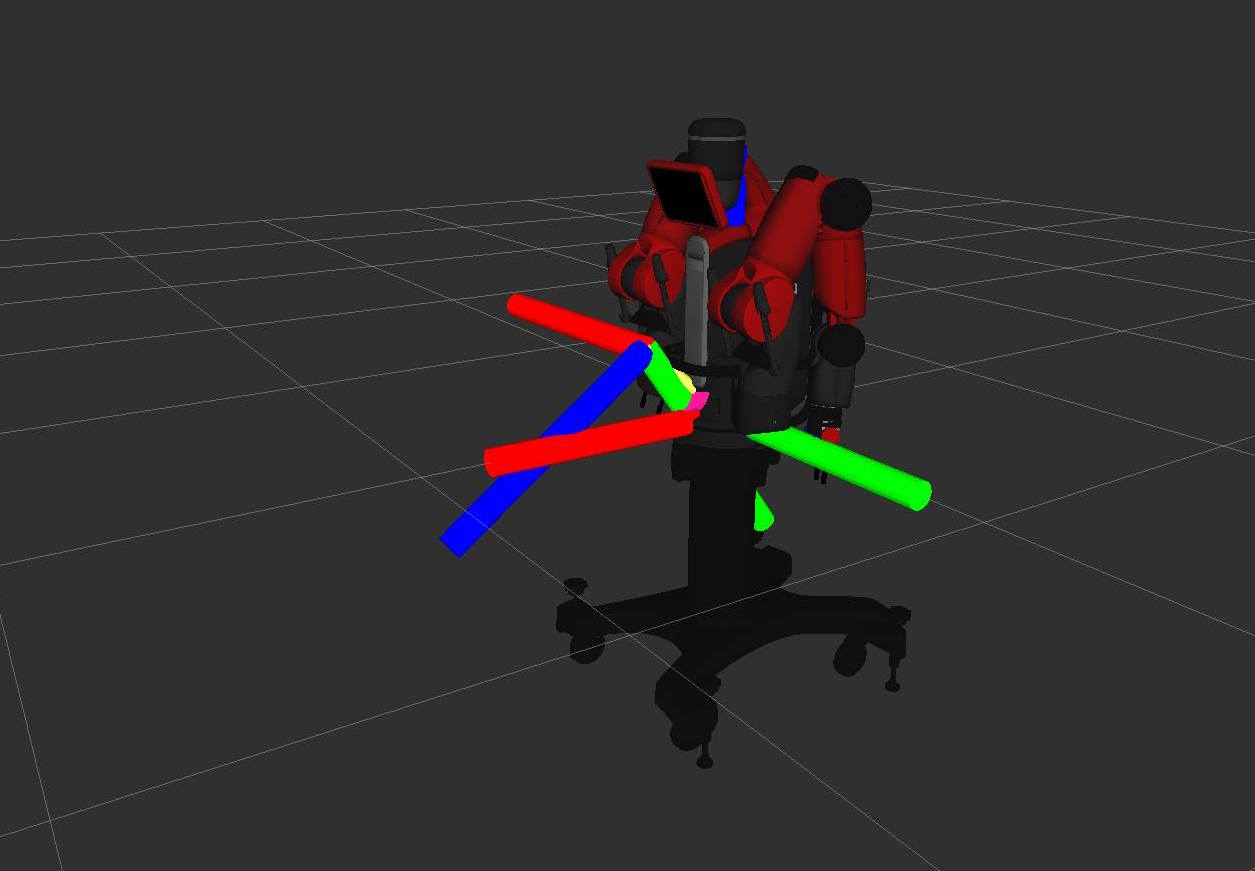
\includegraphics[width = 10cm, height = 6.5cm]{fixedframe.jpg}
\captionof{figure}{\textit{Image showing axes transforms between the Kinect and Baxter's torso frame}}
\bigskip
\end{minipage}
\hspace{0.5cm}
\begin{minipage}{0.29\textwidth}
\raggedright
Fixed coordinate systems were constantly used in testing the vision systems in this project, mainly within rViz. Everytime a coordinate or shape was recognised within the vision system, they could be published to rViz using a PointStamped object, which can be published in a particular coordinate
\end{minipage}
 system. Therefore publishing in one frame, transforming then publishing it another, rViz can show whether a point is correctly detected and whether it is in the correct frame.
\newline
This principle was used in the bowl recognition system, where after the centre of the bowl was obtained, Baxter needed to know where the centre of the bowl was in it's main body coordinate system before a movement command could be made. The system then looked up the transform between the Kinect and Baxter's torso to transform the 3D coordinate between coordinate systems.
\subsection{Custom Service Requests}
The idea that Baxter's movements would all be based on the current states of his vision system - depending upon where both the sweets and the bowl were, there needed to be a method developed for Baxter's movement system to be able to request information from the vision system. This was implemented via Services, which is a method in ROS that allows a custom message to be sent, and then received between two nodes.
% Activate the following line by filling in the right side. If for example the name of the root file is Main.tex, write
% "...root = Main.tex" if the chapter file is in the same directory, and "...root = ../Main.tex" if the chapter is in a subdirectory.
 
%!TEX root =  

\chapter{Methods}
\label{chapter4}
\section{Main ROS Principles}
\subsection{Inverse Kinematics}
dsaokdaskdaskldaskl;dsad
s
d;asdaskldksal;das
dsadsamdaskdkadklas;dsa\newline
lkjsakdsadjksajkdasjldas
\subsection{Visualisation using RViz}
dsaokdaskdaskldaskl;dsad
s
d;asdaskldksal;das
dsadsamdaskdkadklas;dsa\newline
lkjsakdsadjksajkdasjldas
\subsection{Fixed Frame Transforms}
A key aspect of creating the integrated movement system was understanding the concept of fixed frames and transforms. In ROS, Baxter contains information for multiple transforms between every joint and sections of his body. These transforms are known at all times to help know where a point is relative to one part, say the hand, against Baxter's torso. This method works similarly for the Kinect, where Baxter's torso coordinate system, is linked to the Kinect's coordinate system via a transform, which can be accessed by certain methods in ROS.

\begin{minipage}{0.65\textwidth}
\bigskip
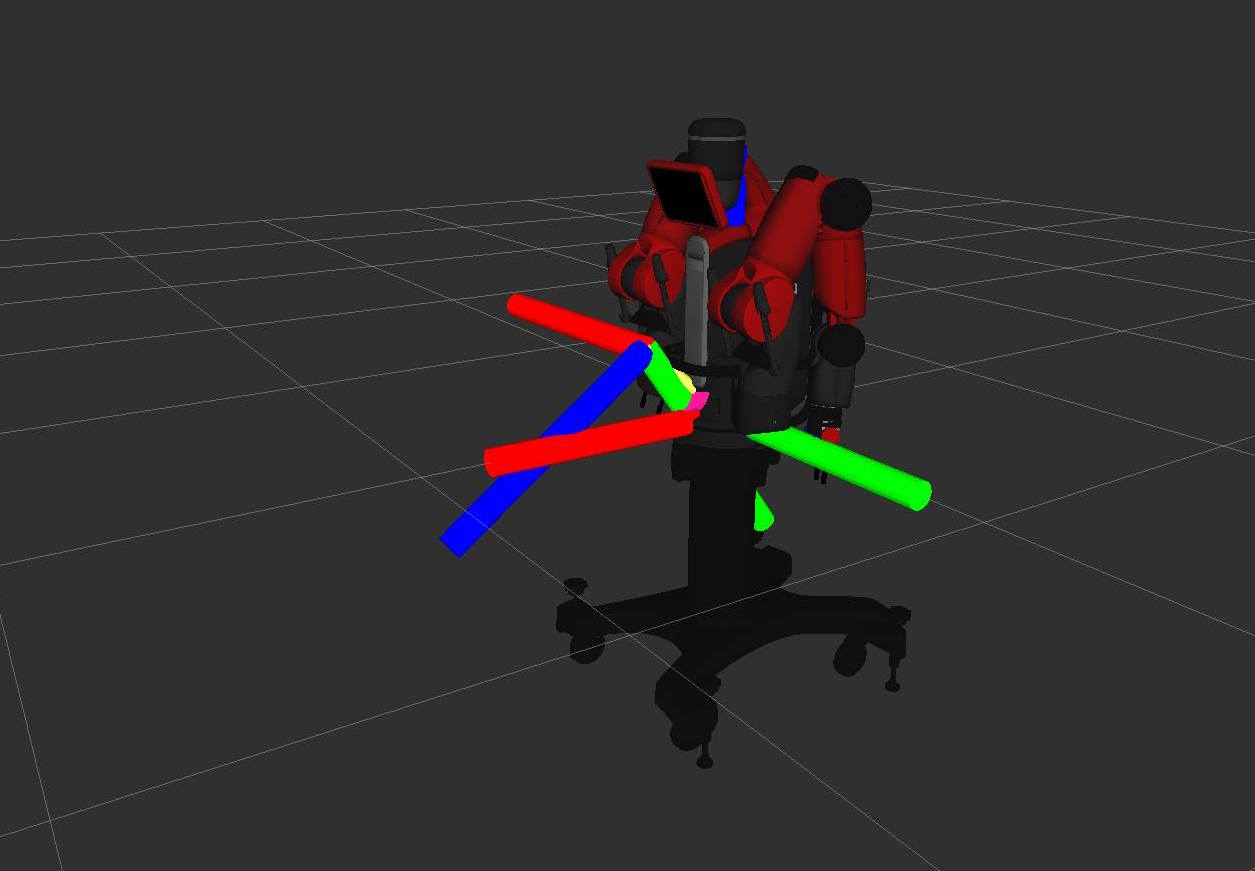
\includegraphics[width = 10cm, height = 6.5cm]{fixedframe.jpg}
\captionof{figure}{\textit{Example RVIZ Image}}
\bigskip
\end{minipage}
\hspace{0.5cm}
\begin{minipage}{0.29\textwidth}
\raggedright
Fixed coordinate systems were constantly used in testing the vision systems in this project, mainly within rViz. Everytime a coordinate or shape was recognised within the vision system, they could be published to rViz using a PointStamped object, which can be published in a particular coordinate
\end{minipage}

 system. Therefore publishing in one frame, transforming then publishing it another, rViz can show whether a point is correctly detected and whether it is in the correct frame.
\newline
This principle was used in the bowl recognition system, where after the centre of the bowl was obtained, Baxter needed to know where the centre of the bowl was in it's main body coordinate system before a movement command could be made. The system then looked up the transform between the Kinect and Baxter's torso to transform the 3D coordinate between coordinate systems.
\subsection{Custom Service Requests}
The idea that Baxter's movements would all be based on the current states of his vision system - depending upon where both the sweets and the bowl were, there needed to be a method developed for Baxter's movement system to be able to request information from the vision system. This was implemented via Services, which is a method in ROS that allows a custom message to be sent, and then received between two nodes.

\section{The Vision System}
\subsection{Calibration and Setup}
\subsection{Basic Vision Techniques}
Throughout this section, there is going to be information on the complex vision techniques used to help Baxter identify the position of the bowl and the sweets on the table. Firstly, here is some background information on the simpler, smaller algorithms used with these:
\begin{itemize}
\item{\textbf{RANSAC} - dsjadsjda}
\item{\textbf{Contours} - dsjadsjda}
\item{\textbf{Gaussian Blurring} - dsjadsjda}
\end{itemize}

\subsection{Bowl Recognition}
\textbf{Pointcloud Segmentation and Recognition}
\newline
The Kinect produces a pointcloud, a set of 3D points in the Kinect's coordinates system. To recognise the bowl of sweets on the table, the vision sytem first separates objects from the points representing the table, then separates those points into individiual object clusters. To eliminate noise and find the bowl cluster, a colour segmentation is performed to find only the white objects on the table. After that, the bowl can then be found by looking for the rim of the bowl as a circle in 3D space. This process is carried out by multiple algorithms, as discussed here:
\newline
\newline
\textbf{1. Tabletop Object Detection/Segmentation} 
\newline
This method works by detecting the main table plane in the Pointcloud by detecting the dominant plane using RANSAC. Points above this plane are then considered to be objects on top of the table, which are then segmented from the points within the table plane. This results in a pointcloud devoid of any points belonging to the table.
\newline
\newline
\textbf{2. Region Growing Segmentation}
\newline
The purpose of this algorithm is to separate the points in the pointcloud into clusters, ones which are close enough to separate into individual objects on the table. The theory behind this algorithm is it takes in the indices and estimated normals of the Pointcloud and for each possible region, calculates a K-nearest neighbour search over the indices. 
\begin{minipage}[t]{0.30\textwidth}
\raggedright
During this search, it compares each point with another, checking first for a specified smoothness constraint, checking if the deviation between normals is within a specified angle. If that is satisfied, then the difference in curvature is tested, allocating the points to the appropriately separated clusters.
\end{minipage}
\hspace{0.5cm}
\begin{minipage}[t]{0.64\textwidth}
\smallskip
\centering
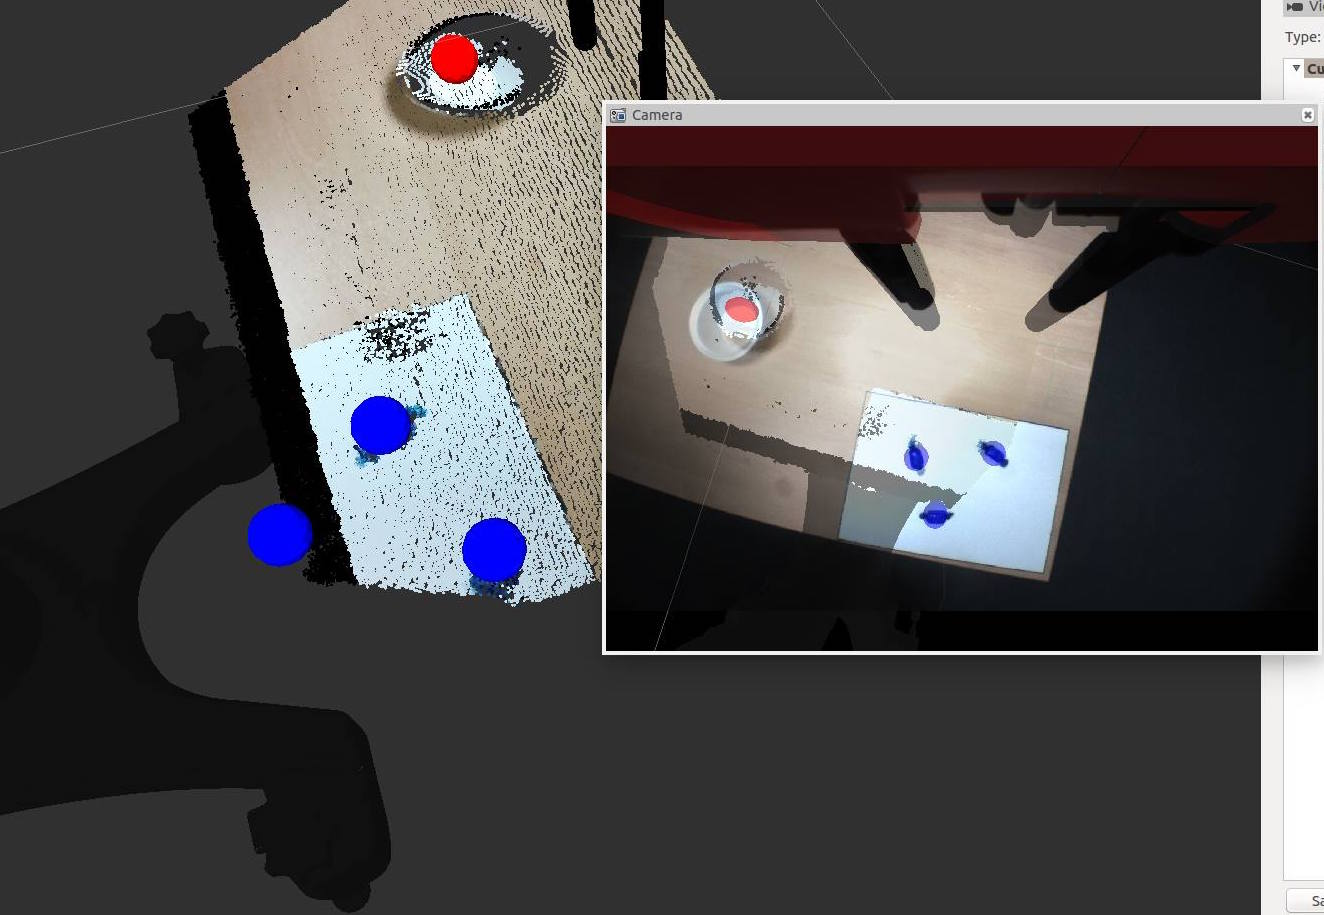
\includegraphics[width = 10cm, height = 6.5cm]{sweettransformation.jpg}
\centering
\captionof{figure}{\textit{An example of segmented objects}}
\bigskip
\bigskip
\end{minipage}
During the implementation of this algorithm, multiple number of neighbours, smoothness and curvature constraints were used until the individual objects in the pointcloud were sufficiently separated.
\newline
\newline
\textbf{3. Colour-Based Segmentation}
\newline
After separation of the Pointcloud into object clusters, a key thing to do was to get rid of noise caused by movement of Baxter's arms in front of the Kinect. 
\begin{minipage}[t]{0.64\textwidth}
\smallskip
\centering
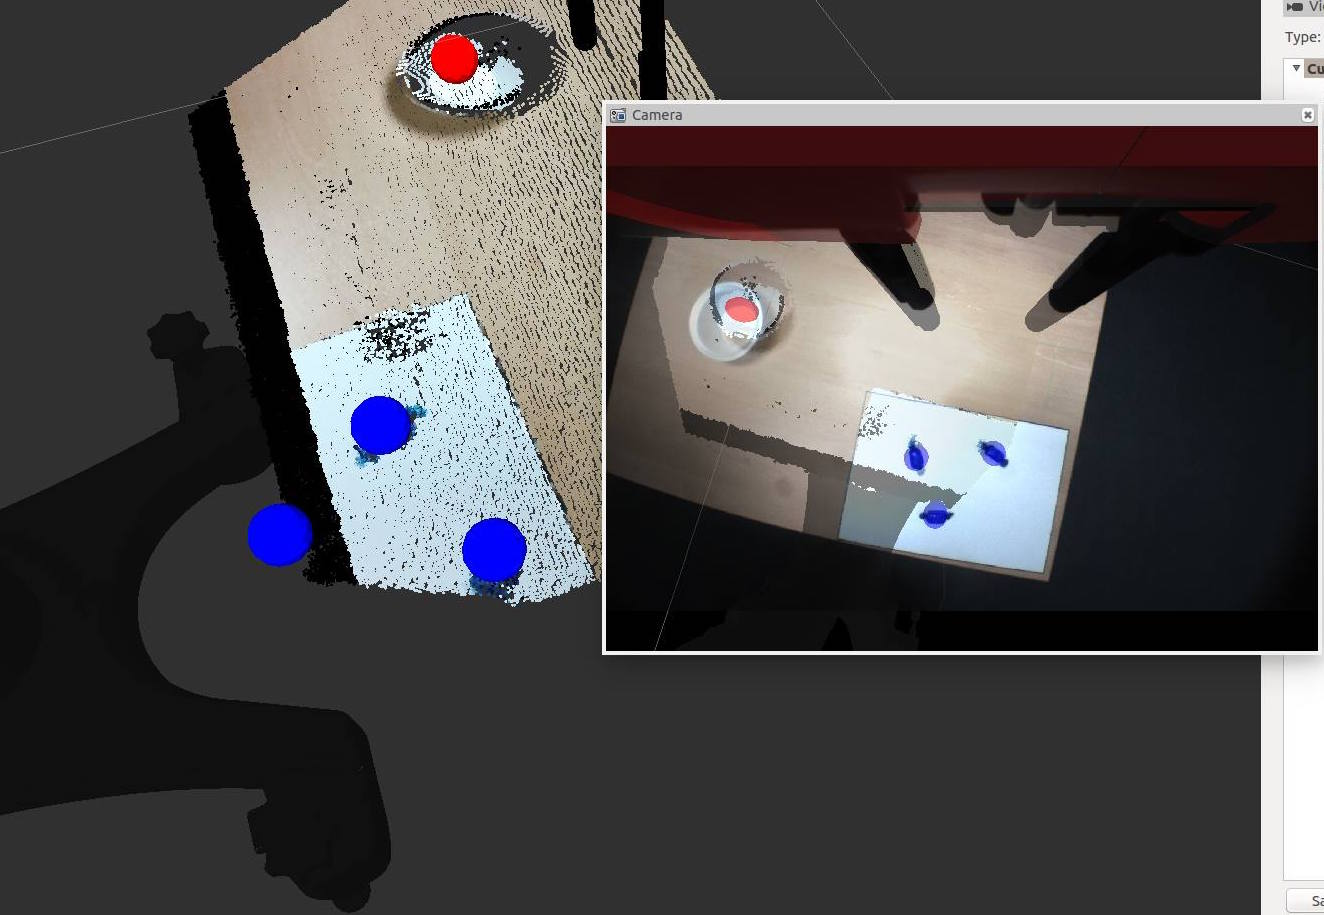
\includegraphics[width = 10cm, height = 6.5cm]{sweettransformation.jpg}
\centering
\captionof{figure}{\textit{An example of white colour segmented objects}}
\bigskip
\end{minipage}
\hspace{0.5cm}
\begin{minipage}[t]{0.29\textwidth}
\raggedright
To do this, black noise/points were eliminated by segmenting the objects further by colour. This was done by looping over the points in each cluster and averaging the RGB values of each cluster. Then, only the white clusters (those with a high enough R, G and B threshold), were
\end{minipage}	
segmented out so that the Pointcloud contains only the points for the bowl and any other white object on the table. This method could be expanded to recognise other colour bowl relatively easily, by finding the correct thresholds for other colour bowls.
\newline
\newline
\textbf{4. Detection of the Bowl Rim}
\newline
The most significant part of the bowl that tended to show up in the PointCloud was the bowl's rim. From that information, it was decided that the simplest solution was to find the rim of the bowl by finding a specific sized circle within a plane of the 3D PointCloud. This method was implemented by using the RANSAC algorithm to detect the points that best fit a circle shape within any plane. This method in the PCL library is especially good at allowing variation in it's detection. By varying distance thresholds and minimum/maximum circle radius values, the bowl was able to be found successfully, even with gaps in the rim, which occurred when Baxter's hands went in front of the bowl. After the circle model had been found in the white PointCloud, the x, y z of the centre of the bowl's rim was then known in the Kinect's frame coordinates.
\newline
\newline
\textbf{5. Improvement on Detection}
\newline
Due to the noise in the Kinect's Pointcloud recordings, some improvements were made further into development. The problem with the circle detection was that noise caused the centre of the bowl to shift each frame. To counteract the noise in detection, a cumulative average was taken over 20 frames and outputted as an average bowl centre. Then a cumulative centre point was taken further over time to de-noise the results, resulting in a fixed bowl centre that Baxter could reliably use as the actual centre of the bowl on the table.
\subsection{Sweet Recognition}
The task of Baxter recognising the sweets involved him being able to look at an area of the table with sweets retrieved from the bowl and determine how many sweets there were in that area along with what type/colour each sweet was. The problem with recognising the sweets using the Kinect is that the sweets were such small objects, that the noise in the Kinect meant that a significant number of sweets weren't picked up after segmenting objects on the table. Therefore an alternative method was proposed using OpenCV. The idea behind this method was for Baxter to capture an image of the table with the sweets on using his hand camera. Then from that image, OpenCV image processing techniques could be applied to separate the sweets into individual objects, from which the shapes, centres and colours could be obtained.
\newline\newline
The first task in separating the sweets was to have Baxter to only look in the area the sweets were placed on the table, so the sweets remaining in the bowl would not interfere. It was decided that the easiest way to segment this area out was to use a white piece of paper as the background, making it easier to segment out the rest of the image. The piece of paper used was A3 in size and had a black edge drawn on, to help detect the border of the page. Multiple vision methods were trialled to try and recognise this sweet placement area, explained here:
\newline
\newline
\textbf{Image Pre-processing}
\newline
\begin{minipage}[t]{0.30\textwidth}
\raggedright
\smallskip
Before the image from the camera could first be used, some pre-processing was taken place to reduce noise and make it easier to detect the area on the table. A Gaussian Blur was performed with a small kernel to firstly blur the image to reduce possible noise. Then, Canny Edge Detection was used to detect edges within the image, along 
\smallskip
\end{minipage}
\hspace{0.5cm}
\begin{minipage}[t]{0.64\textwidth}
\smallskip
\centering
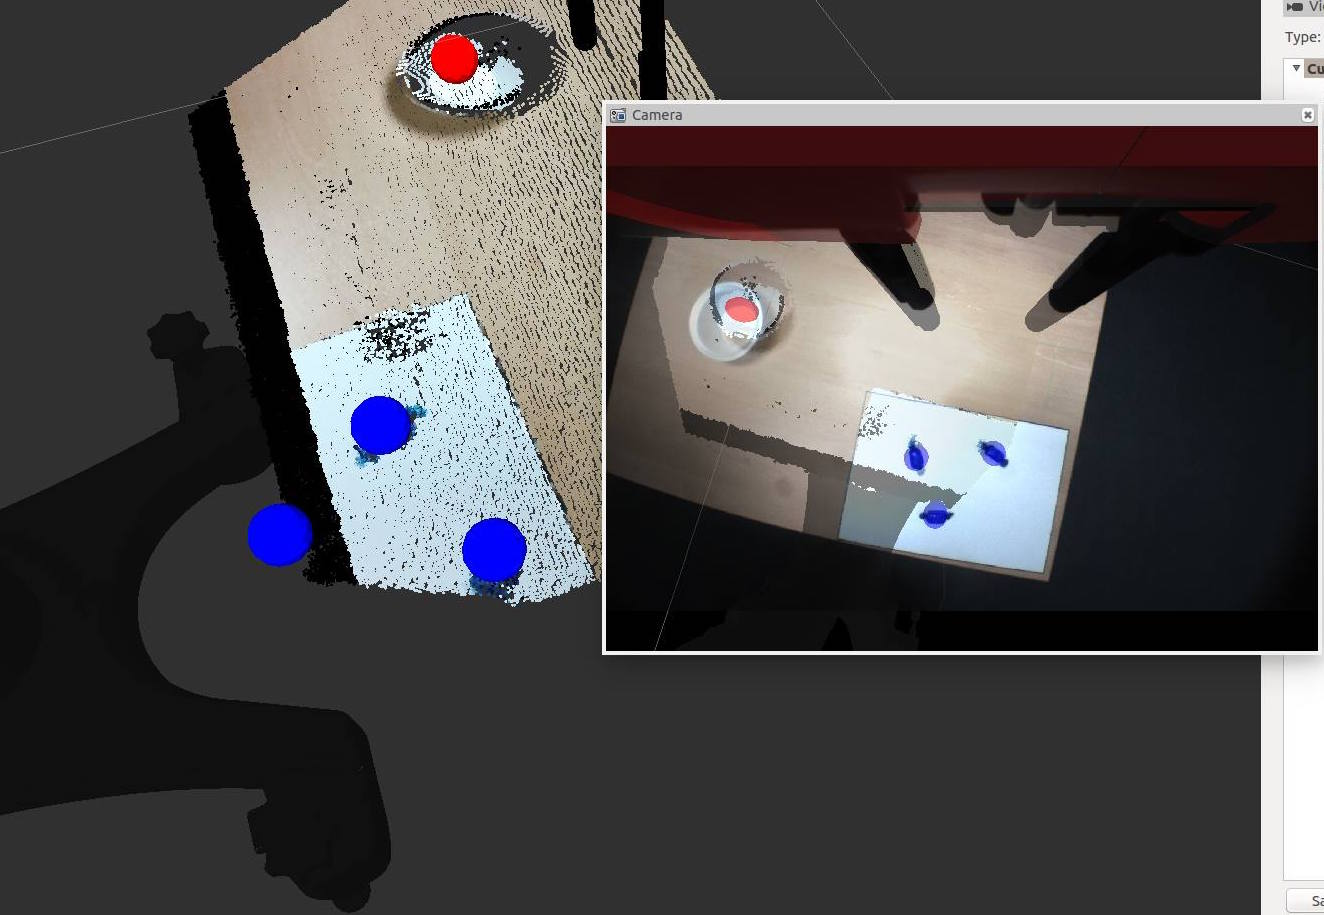
\includegraphics[width = 10cm, height = 6.5cm]{sweettransformation.jpg}
\centering
\captionof{figure}{\textit{An example of segmented objects}}
\bigskip
\end{minipage}
with dilation and erosion to close any incomplete edges, resulting in a reasonably successful edge detection for the entire image.
\newline
\newline
\begin{minipage}[t]{0.30\textwidth}
\raggedright
\smallskip
\textbf{Hough Line Transform}
\newline
Firstly, to find a rectangle in the image, Hough Line Transform was attempted to be used to find the individual edges of the paper. This technique was somewhat successful when attempting to distinguish between the edges however, by varying and optimising the line detection threshold, 
\smallskip
\end{minipage}
\hspace{0.5cm}
\begin{minipage}[t]{0.64\textwidth}
\smallskip
\centering
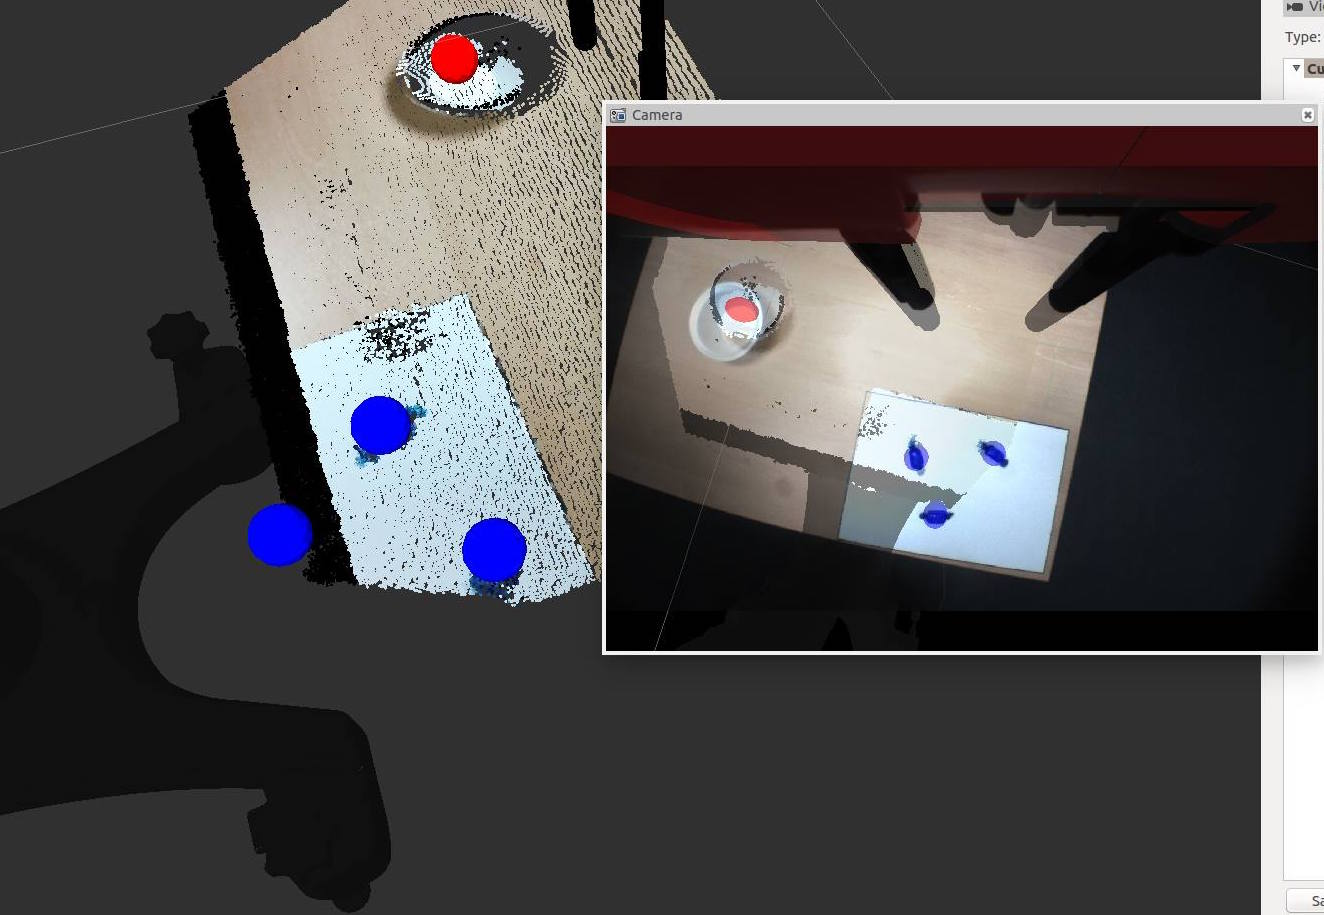
\includegraphics[width = 10cm, height = 6.5cm]{sweettransformation.jpg}
\centering
\captionof{figure}{\textit{An example of segmented objects}}
\bigskip
\end{minipage}
it was difficult to detect all four edges of the paper constantly. Either one or two edges kept being detected then undetected or too many edges were found. Due to the inaccuracy of this edge detection, the four edges could not always be found to form the rectangle. Therefore other methods were explored.
\newline
\newline
\textbf{Contour Detection}
\newline
\begin{minipage}[t]{0.64\textwidth}
\smallskip
\centering
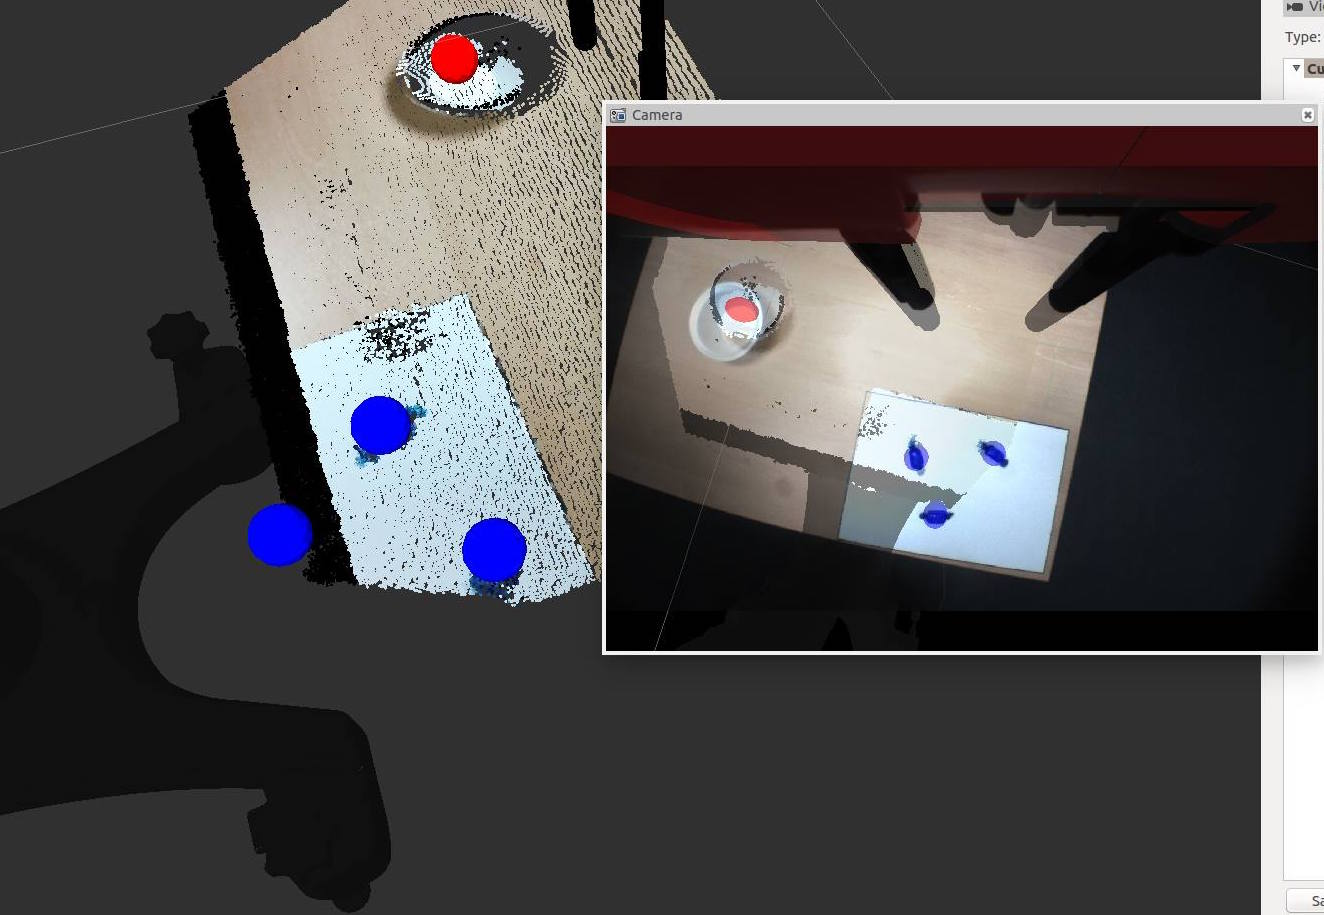
\includegraphics[width = 10cm, height = 6.5cm]{sweettransformation.jpg}
\centering
\captionof{figure}{\textit{An example of white colour segmented objects}}
\bigskip
\end{minipage}
\hspace{0.5cm}
\begin{minipage}[t]{0.29\textwidth}
\raggedright
Once the black border on the area was defined enough to be consistent during canny edge detection, a contour successfully managed to detect the four edges of the paper. Due to there being many contours detected in the image, certain constraints had to be put on the detection to segment out the sweet 
\end{minipage}	
area. The main method of segmenting out the rectangular area then was to first eliminate the smaller contours by size (using the in-built countourArea) and then approximate a polygon for the countours to detect which countour was a rectangle. This contour then produced a mask, which could segment out the rest of the image from the sweet area.
\newline
\newline
Once the sweet placement area was reliably segmented out from the image, multiple methods were used to attempt to try and identify the individual sweets. These methods are explained below:
\newline
\newline
\begin{minipage}[t]{0.30\textwidth}
\raggedright
\smallskip
\textbf{Hough Circle Transform}
\newline
For the simple, round sweets initially used in trials, a Hough Circle detection algorithm seemed like a sensible way to detect the simpler, round sweets. However, like the Hough Line detection used earlier, it was hard to get a constant solution, with circles  
\smallskip
\end{minipage}
\hspace{0.5cm}
\begin{minipage}[t]{0.64\textwidth}
\smallskip
\centering
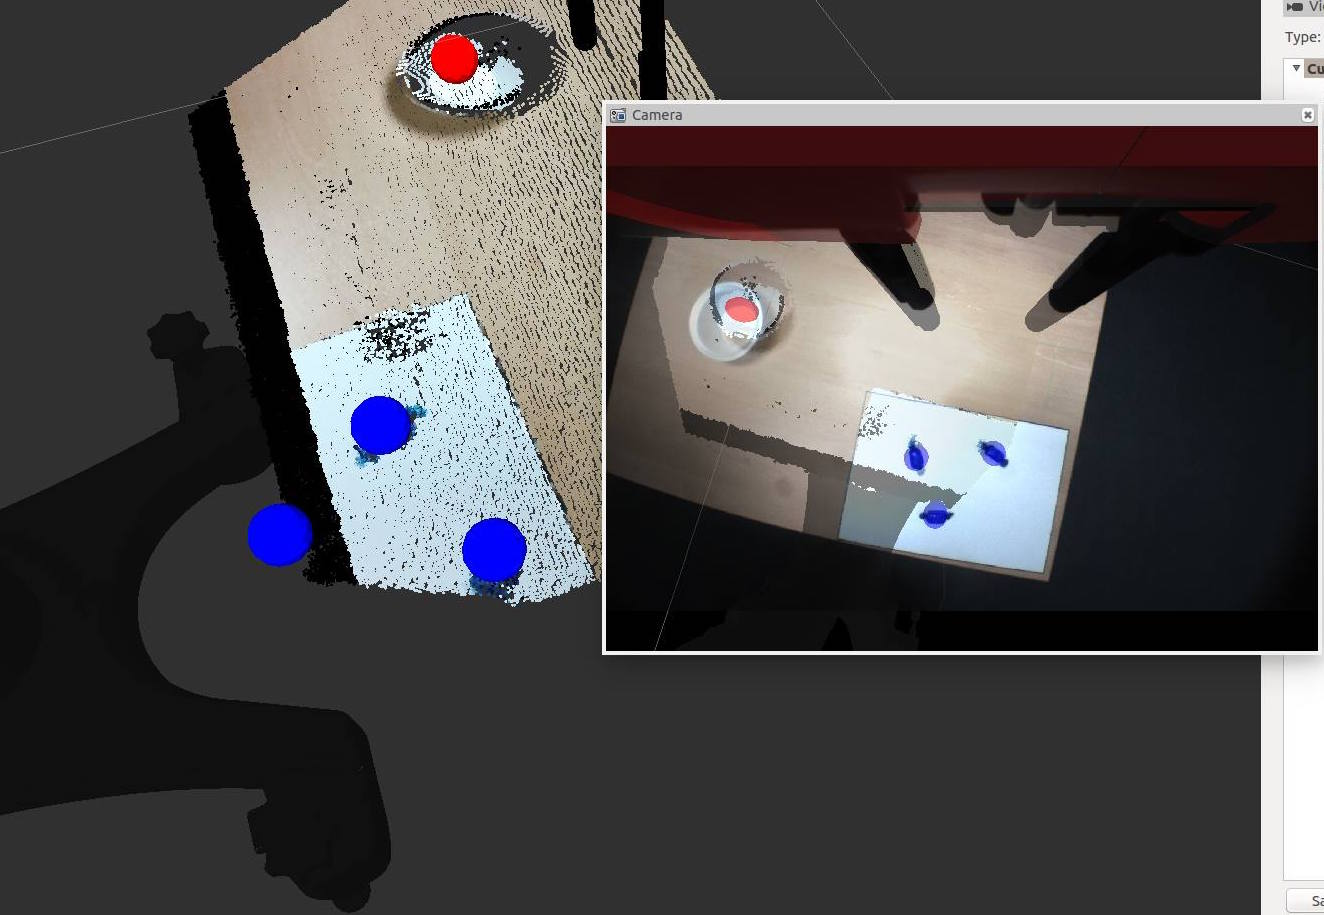
\includegraphics[width = 10cm, height = 6.5cm]{sweettransformation.jpg}
\centering
\captionof{figure}{\textit{An example of segmented objects}}
\bigskip
\end{minipage}
being detected and then undetected throughout various received image frames, therefore other methods needed to be tried to get a more reliable vision system.
\newline
\newline
\textbf{Contour Detection}
\newline
A better method was to do some image processing, Gaussian blurring, closing and opening to produce a lot better results, producing a mask of a white background with some black sweets in front. The problem with using this method is due to reflections on the sweets wrappers, this caused an issue of multiple broken contours within an individual sweet, whereas a preferred method would have been to capture the whole sweet with one contour, as Baxter needs to be able to count each sweet once.
\newline
\newline
\textbf{HSV Colour Segmentation with Contour Detection}
\newline
\begin{minipage}[t]{0.64\textwidth}
\smallskip
\centering
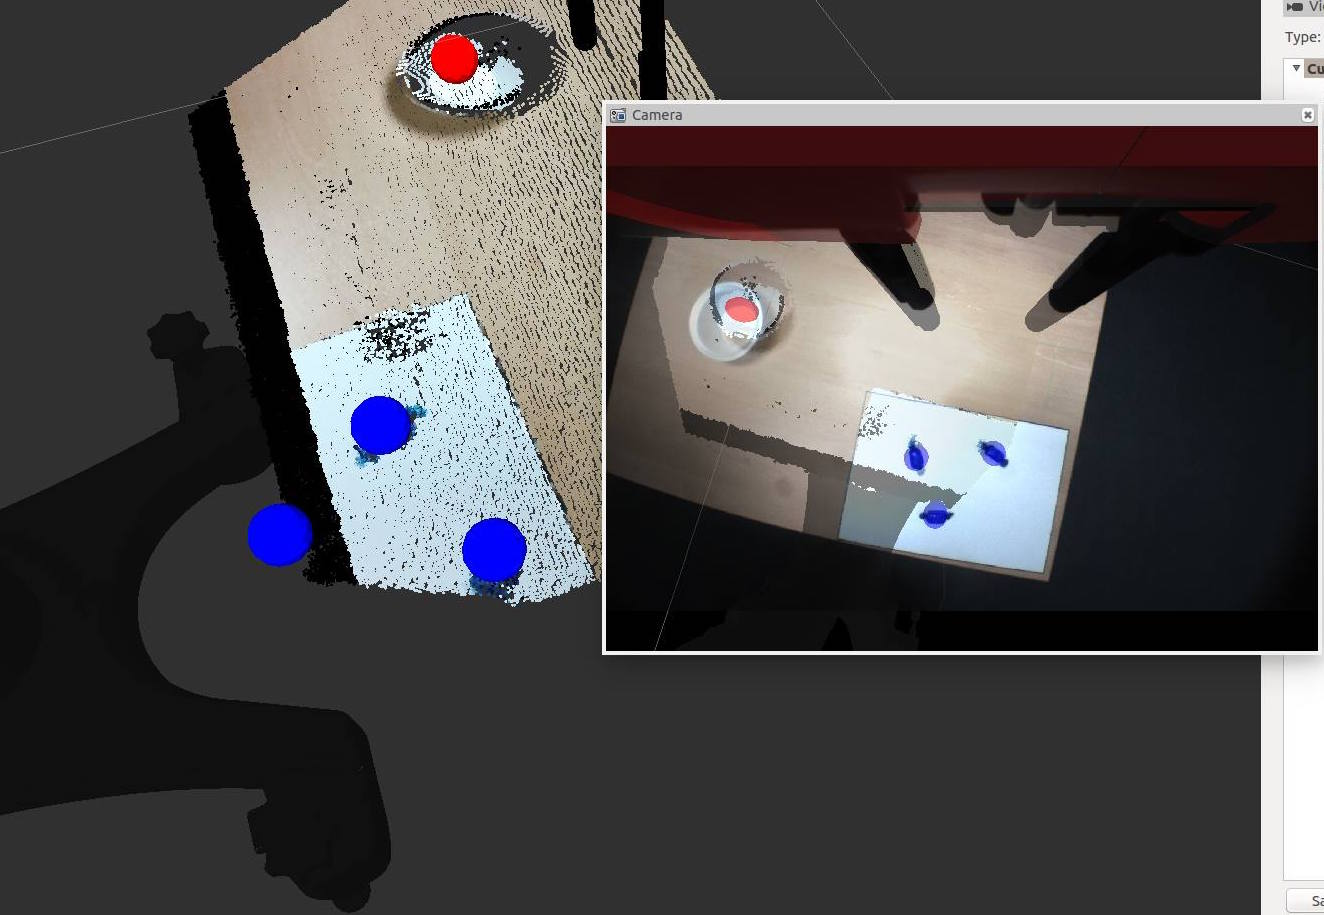
\includegraphics[width = 10cm, height = 6.5cm]{sweettransformation.jpg}
\centering
\captionof{figure}{\textit{An example of white colour segmented objects}}
\bigskip
\end{minipage}
\hspace{0.5cm}
\begin{minipage}[t]{0.29\textwidth}
\raggedright
A more accurate method was found by using an existing tool called objectfinder. This tool uses multiple sliders to segment an image and produce a mask using lower and upper bounds for RGB values. Since each sweet wrapper had different identifiable colours and they were placed onto a separatable 
\end{minipage}	
white background, using a scale of possible HSV values could be used to identify main sweet wrapper colours - blue, green, red etc. The only limitation of this approach was that similar colours under light could be mixed up, for example, red and pink wrappers had overlapping HSV RBG ranges, and therefore could not be both separated and identified by this method. It did however result in very clear contours for the significantly different colours so this method was used for the sweet recognition. Possible improvements could be made with shape recognition then colour analysis, which may have been able to identify a typical sweet shape and then separate by colour after.
\newline
\newline
Now there was a method for the sweets to be detected, by extracting moments from the sweet contours, the 2D pixel coordinate could be retrieved from the 2D image. The problem then was converting the 2D points in that image into 3D world coordinates. 
This was done using an altered version of a pinhole camera method, where the u, v coordinate within the 2D image could be converted to a 3D world coordinate using Baxter's in-built calibrated camera matrix. The equation uses the x and y camera offset values, with the focal lengths to scale the initial point. Then using the distance from the camera to the table (which is fixed), the points can then be converted into 3D world coordinates. This was tested using rViz and Baxter to make sure it worked.
\subsection{Sweet Singulation}
\section{The Manipulation System}
\subsection{Manipulating the Bowl}
\subsection{Sweet Manipulation}
\section{Human Interaction}
\subsection{Voice Recognition}
\subsection{Hand Recognition}
Pages to be referenced for practical applications:
\newline
\url{http://docs.opencv.org/3.0-beta/doc/py_tutorials/py_imgproc/py_houghlines/py_houghlines.html#py-hough-lines}
\url{http://docs.opencv.org/2.4/modules/calib3d/doc/camera_calibration_and_3d_reconstruction.html}
\url{http://pointclouds.org/documentation/tutorials/region_growing_segmentation.php}
\newline
\url{http://pointclouds.org/documentation/tutorials/region_growing_rgb_segmentation.php}
\newline
\url{http://wiki.ros.org/tabletop_object_detector}
\newline
\url{http://docs.pointclouds.org/trunk/group__sample__consensus.html}
\newline
\newline
~\cite{kinectfusion}
~\cite{objectlabelling}
~\cite{herbrobot}
~\cite{reliablegrasping}
\chapter{The Integrated System}
\label{chapter5}
Throughout the methods being developed and tested, they had to be added and integrated together into an overall system. This chapter describes the process taken to integrate all of the features together by using service communications, roslaunch files and basic logic to create the final product.
\section{Feature Integration}
After the features had been developed from the Methods section, a major challenge was to integrate all of these features to work together in the shop environment. This was done by first moving the code from all the manipulation tasks into one file\footnote{Github repository: Manipulation - shopkeeper.py. \url{https://github.com/um10kh/baxter-project/blob/master/src/manipulation/src/robot_shopkeeper_nk.py}} to allow the shopkeeper to be able to do all the manual tasks required. These manual tasks were commented clearly and placed under the \textit{Shopkeeper} class.
\newline\newline
Once, Baxter was able to carry out the manual tasks such as tilting the bowl and grabbing sweets, the next task was to integrate a communications system (using the \textit{Communications} class), to connect the main Shopkeeper node with the vision/other nodes. The main method of doing this was with custom service messages, where the Shopkeeper node would launch a service, sending a custom message, using a .srv file structure. The Shopkeeper node would then wait for an appropriate response returned from another node, before retrieving the information and using it. An example of this would be when Baxter was waiting for a customer to appear. He would look where he expected a customer then send the \textit{find\_person} node a message to find the next customer. That node would then wait for a customer to approach Baxter and wait in front of the camera, before sending a confirmation message back to the main node. This principle was used on the other aspects of the system too, such as finding the bowl, finding the sweets on the table and receiving voice commands from the Android application.
\subsection{Roslaunch Files}
Once all of the code and communications had been integrated into one file, a roslaunch file\footnote{Github repository - Launch - shopkeeper.launch. \url{https://github.com/um10kh/baxter-project/blob/master/src/manipulation/launch/shopkeeper.launch}} was built to help make the setup of the software more simple. Without a roslaunch file, the system had to be run by starting specific nodes at specific times, with around 9 different terminals running at the same time. The idea of this file was for there to only be one command to launch them all at the appropriate time, for ease of setup and testing. The basic approach would first launch all of the main Baxter-related nodes such as tucking his arms (so they always start in a fixed position) and opening the right hand camera and head camera with their correct resolutions. Then, the main vision systems were started, looking for the sweet area, the bowl on the table and the customer entry. After that, the application server would be started on the node and the application on the device, meaning the main shopkeeper node could then be run.
\subsection{System Logic}
The roslaunch file meant that all the nodes could run at once however, to make the manipulation and vision tasks fully integrated, some system logic was developed for Baxter to be able to constantly run these nodes, looking for new customers and running the `shop' more intelligently.
\begin{figure}[H]
        \centering 
        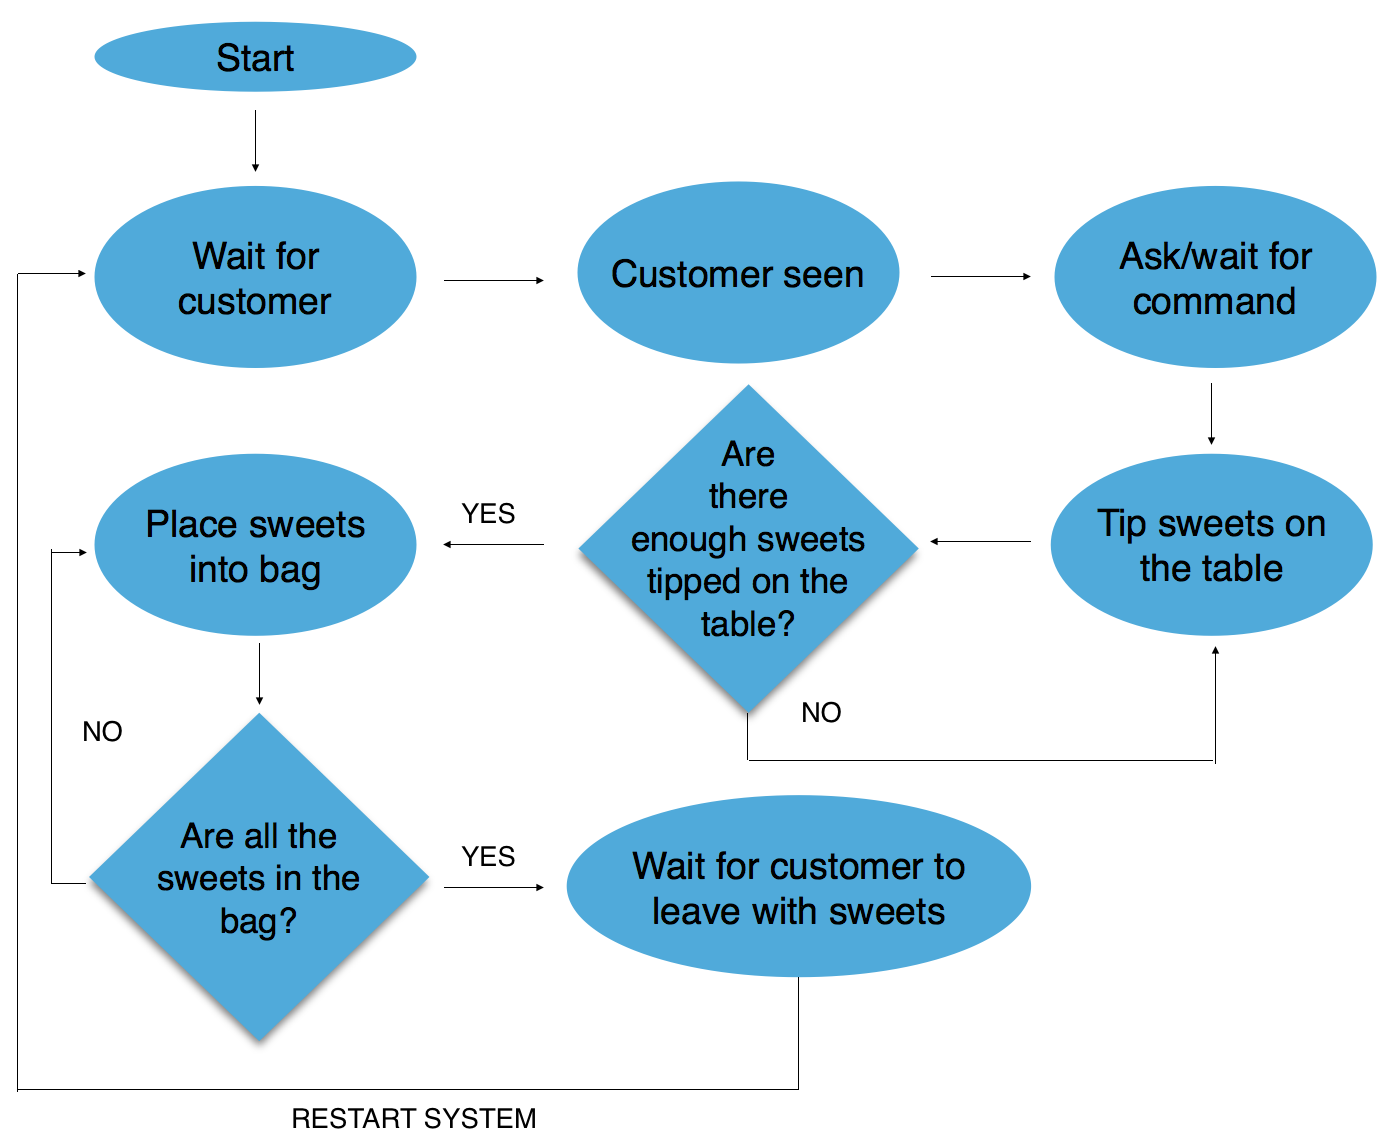
\includegraphics[width=0.75\textwidth, height=10cm]{completesystemlogic.png}
        \caption{A flow chart showing the overall system logic used to build the integrated system.}
         \label{fig:fakegripper}
\end{figure}
The key way to implement the logic was to develop the code around the major decision points. The basic way to do this was to implement while loops with logic checks. For example, a while loop would start, checking the sweets on the table using the sweet vision system. Then if there weren't enough sweets, Baxter would keep looping the code,  tipping the bowl continually onto the table until there were enough sweets, which would  break out of the loop. This principle was used for all the major decision points in the logic system and a `while True' loop was placed round the whole system so once a customer had left, the whole system would start again.
\subsection{User Setup}
Once the logic was implemented and the roslaunch file was written, setup options were added to the start of the program to make it easier for the user to start the system. Since there was no bag/sweet container recognition developed, I implemented a setup function that would prompt the user to place the right arm over the sweet bag and press enter, saving the joint positions so Baxter knew where to drop the sweets. Other user prompts for user setup were made in the same way. The user was prompted to open the android app and enter the shared IP address from the terminal and to place the gripper onto the table to retrieve the table's z height.
\newline\newline
An issue that arose towards the end of the system was when Baxter tried to grab some sweets, the inverse kinematics system caused his arm to knock off and break the clamp/stand for the Kinect attached to his torso. To get by this, a roslaunch file was created to ignore the bowl detection nodes and the user setup prompted the user to move the bowl underneath Baxter's gripper. This helped to test the overall system without having to use the Kinect. The user setup README\footnote{Github repository: User README. \url{https://github.com/um10kh/baxter-project/blob/master/README.md}} explains how the user could setup the system with or without the use of a Kinect.
\section{Integrated System Images}
Once the integration had been implemented along with the user setup, it was then time to test the final system. Firstly, a video taken to demonstrate the capabilities of the system. Stills from this video\footnote{Github repository - Complete System Video. \url{https://github.com/um10kh/baxter-project/blob/master/videos/IntegratedSystemCompressed.mp4}} are provided below in \textbf{\Cref{fig:completeSystem}} and show from (a) to (i) how a generic customer-shopkeeper transaction takes place with Baxter.\newline\newline
In this particular scenario, the customer approaches Baxter and when prompted, asks for one blue, one red and one green sweet. On his first attempt, he tips out the sweets, recognises them and grasps them from the small pile on the left of the page.
\begin{figure}[H]
\makebox[\linewidth][c]{%
\begin{subfigure}[b]{.43\textwidth}
\centering
\caption{}
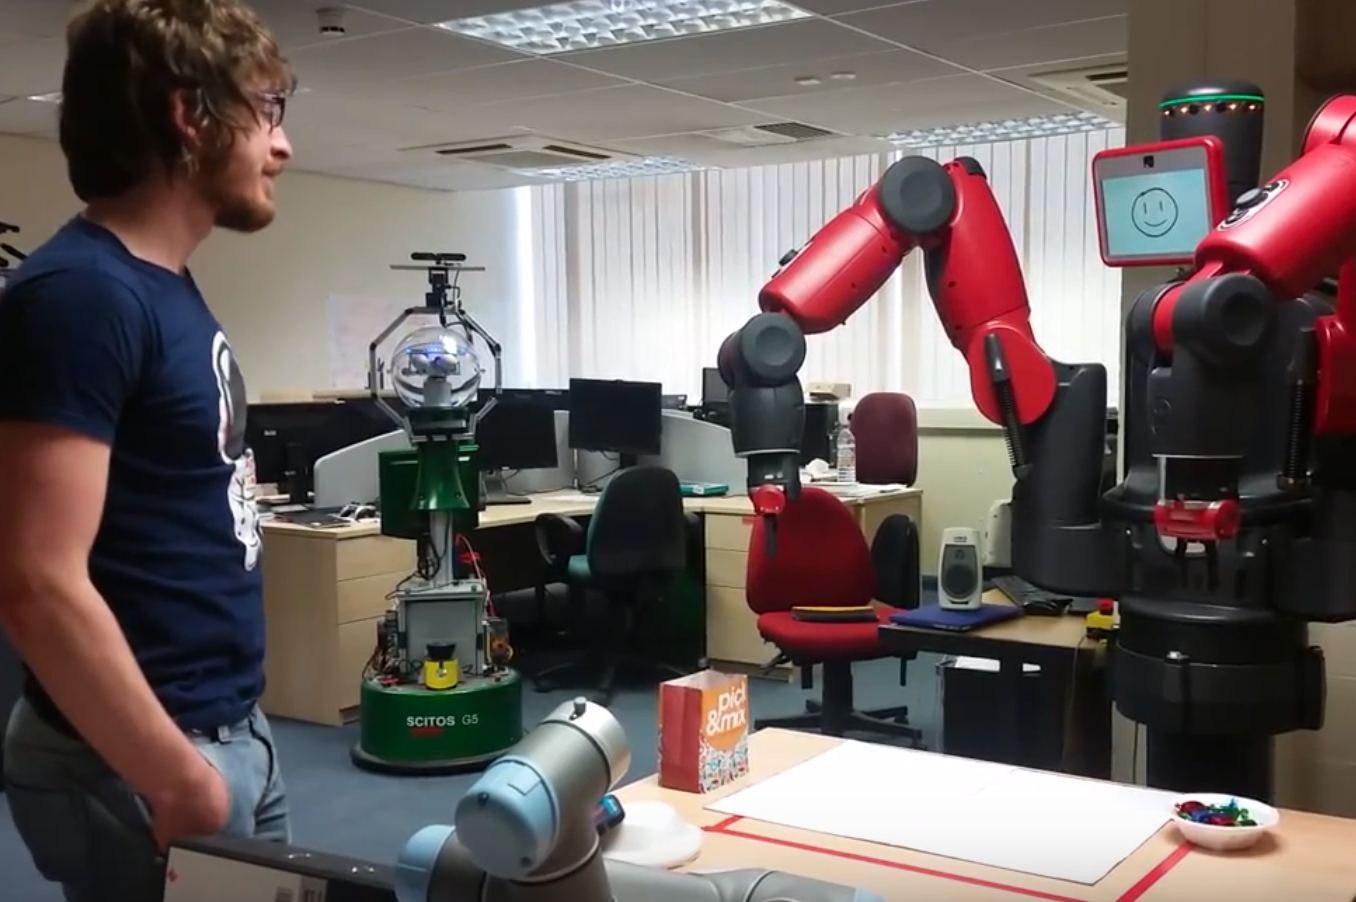
\includegraphics[width=.95\textwidth, height=4.3cm]{1.png}
\end{subfigure}%
\begin{subfigure}[b]{.43\textwidth}
\centering
\caption{}
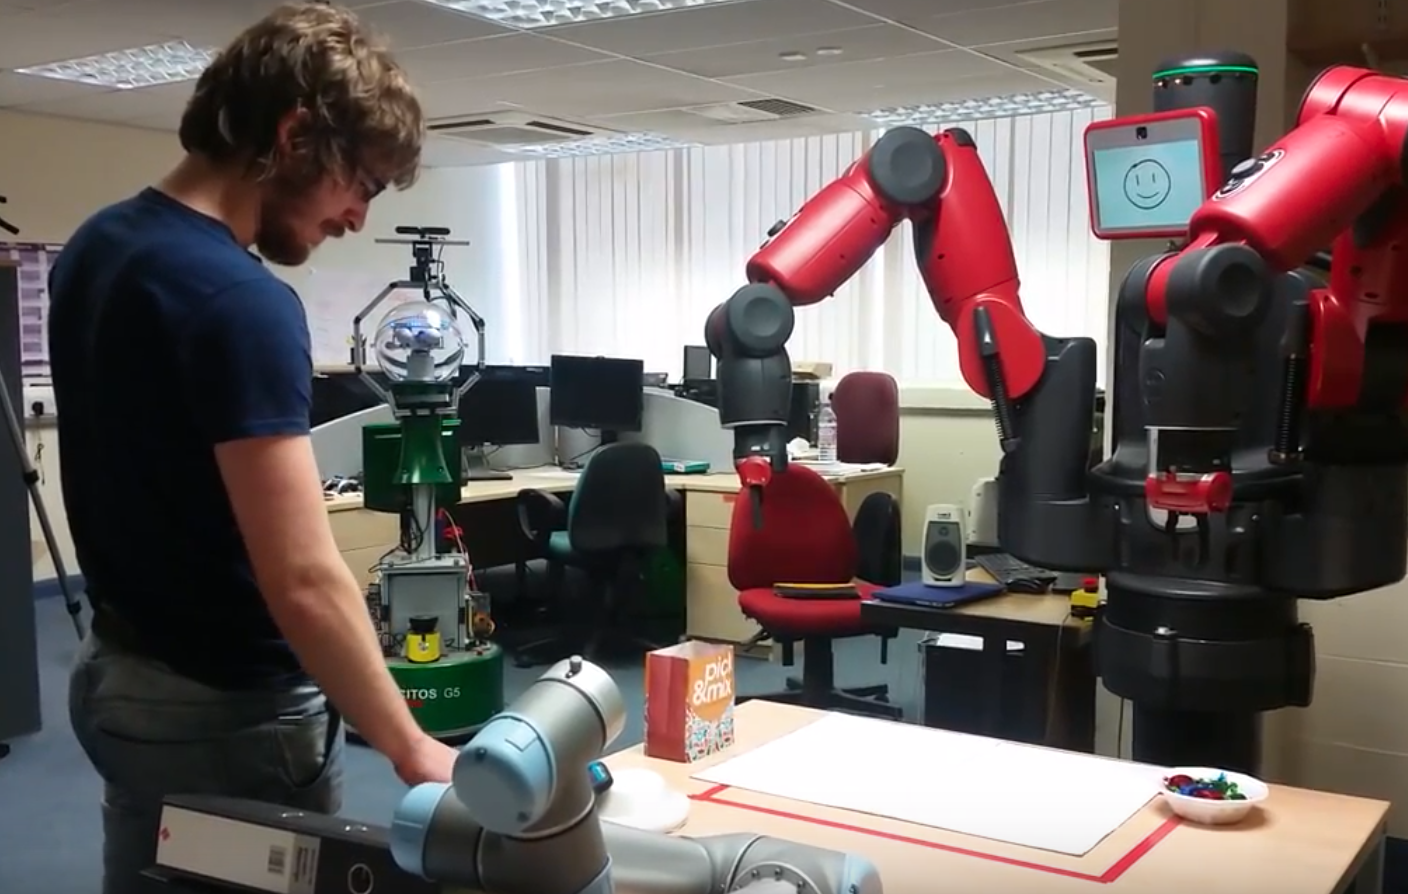
\includegraphics[width=.95\textwidth, height=4.3cm]{3.png}
\end{subfigure}%
\begin{subfigure}[b]{.43\textwidth}
\centering
\caption{}
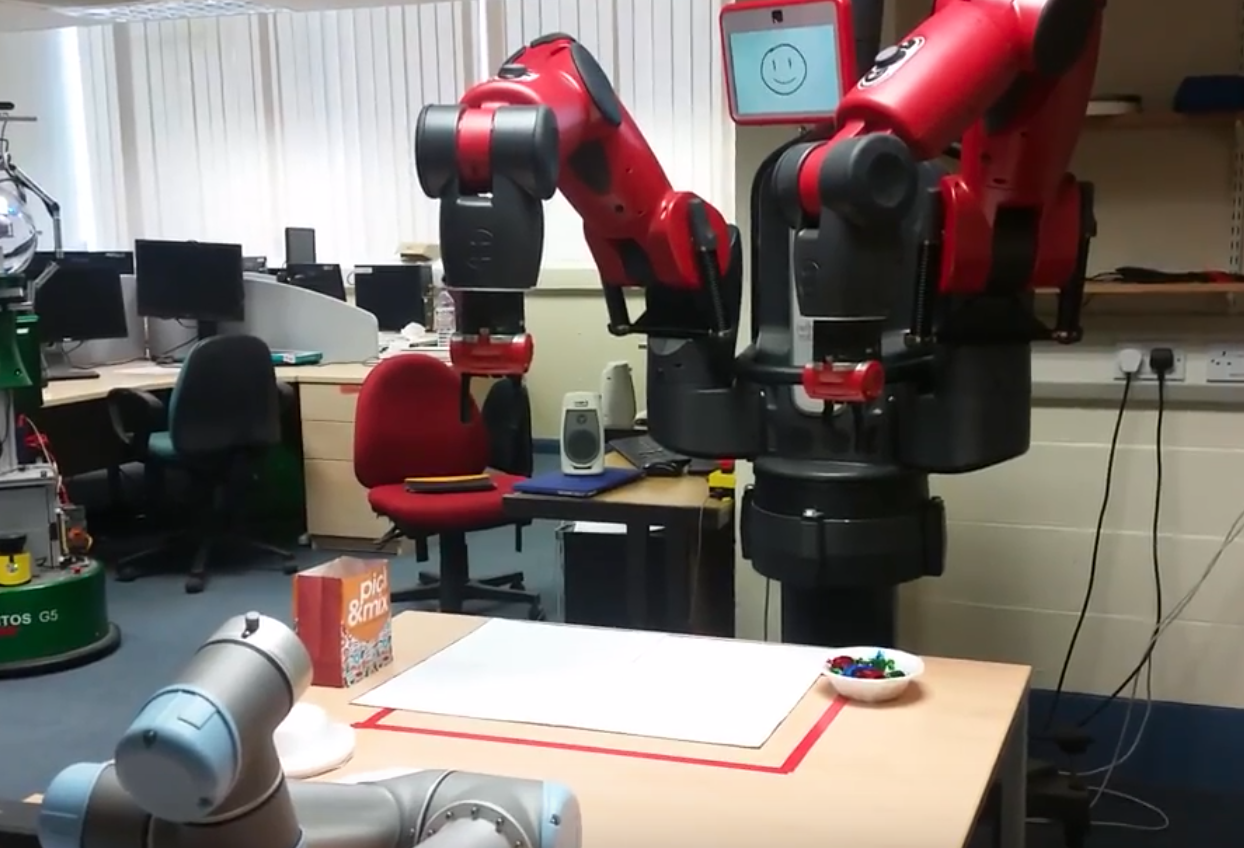
\includegraphics[width=.95\textwidth, height=4.3cm]{4.png}
\end{subfigure}%
}\\
\makebox[\linewidth][c]{%
\begin{subfigure}[b]{.43\textwidth}
\centering
\caption{}
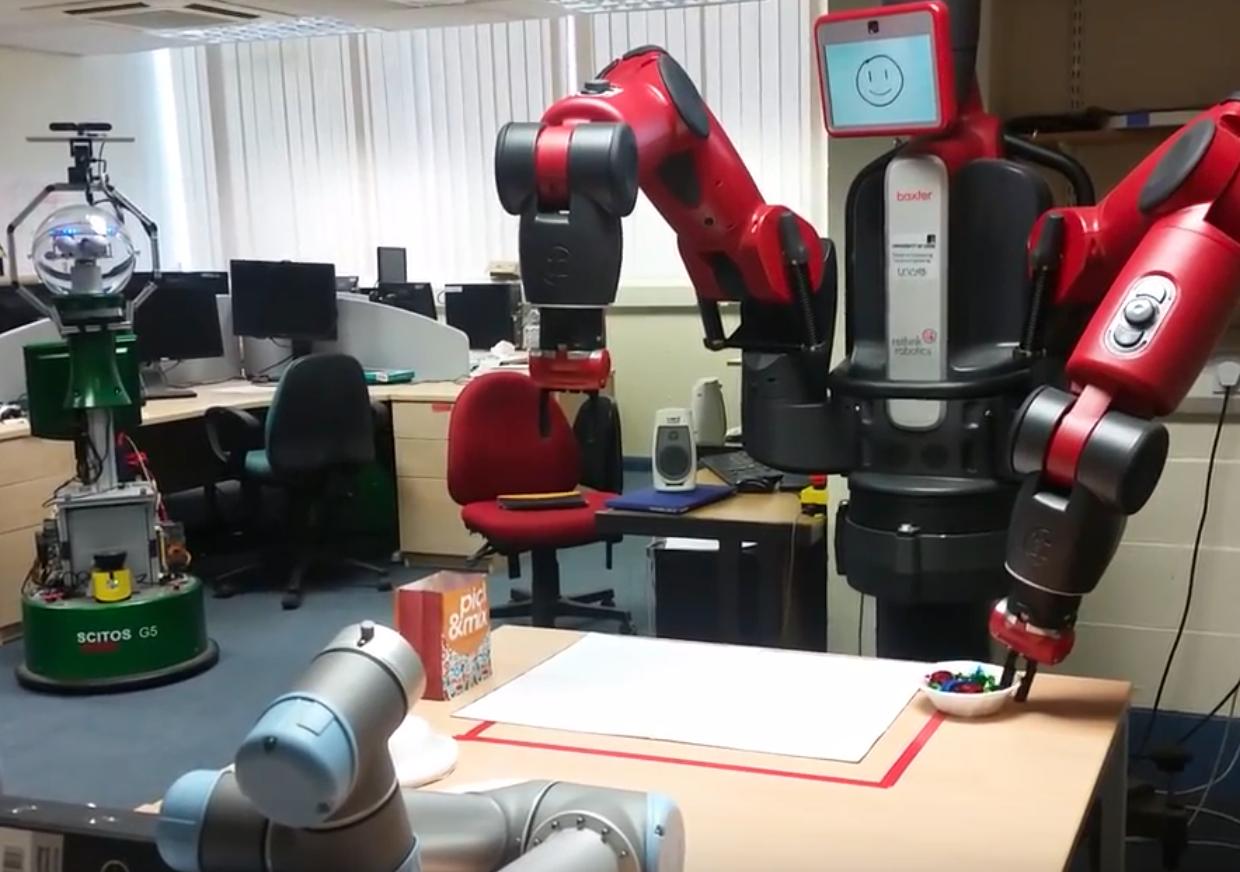
\includegraphics[width=.95\textwidth, height=4.3cm]{5.png}
\end{subfigure}%
\begin{subfigure}[b]{.43\textwidth}
\centering
\caption{}
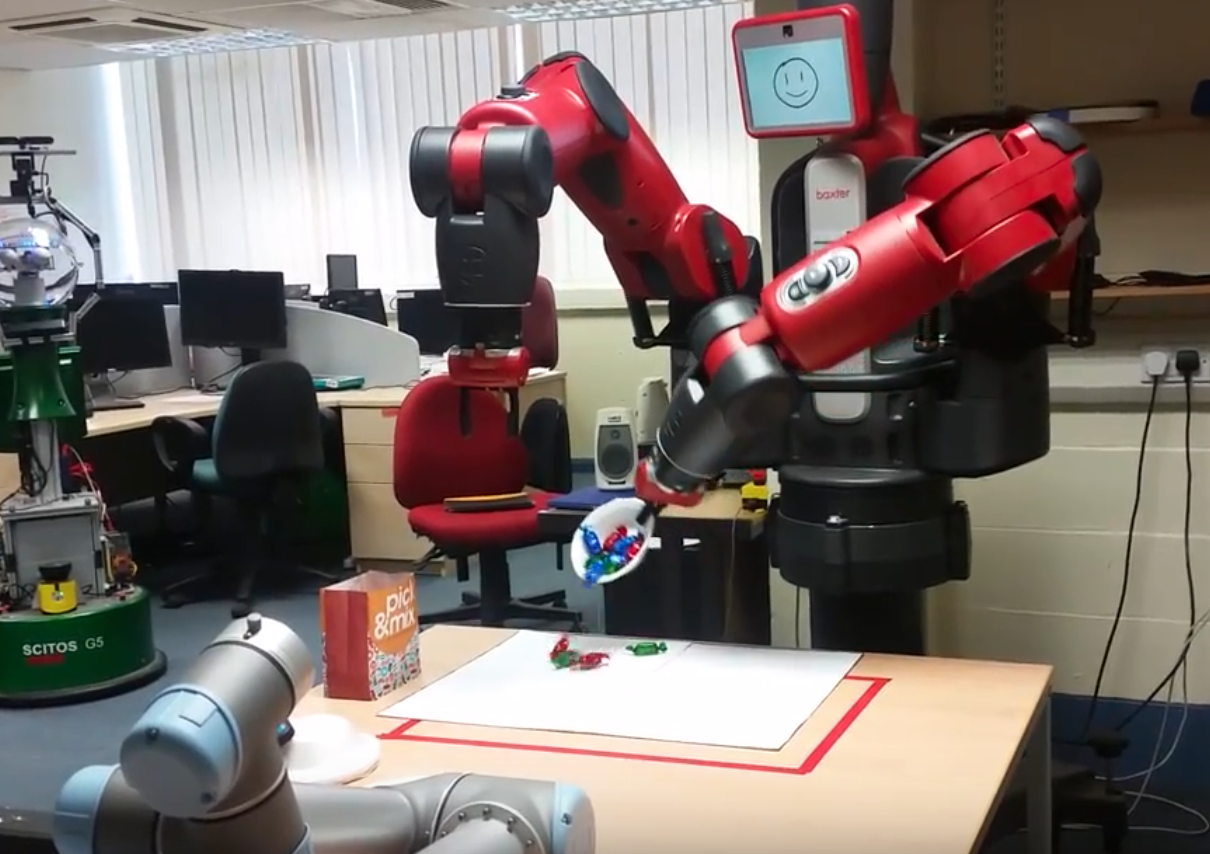
\includegraphics[width=.95\textwidth, height=4.3cm]{7.png}
\end{subfigure}%
\begin{subfigure}[b]{.43\textwidth}
\centering
\caption{}
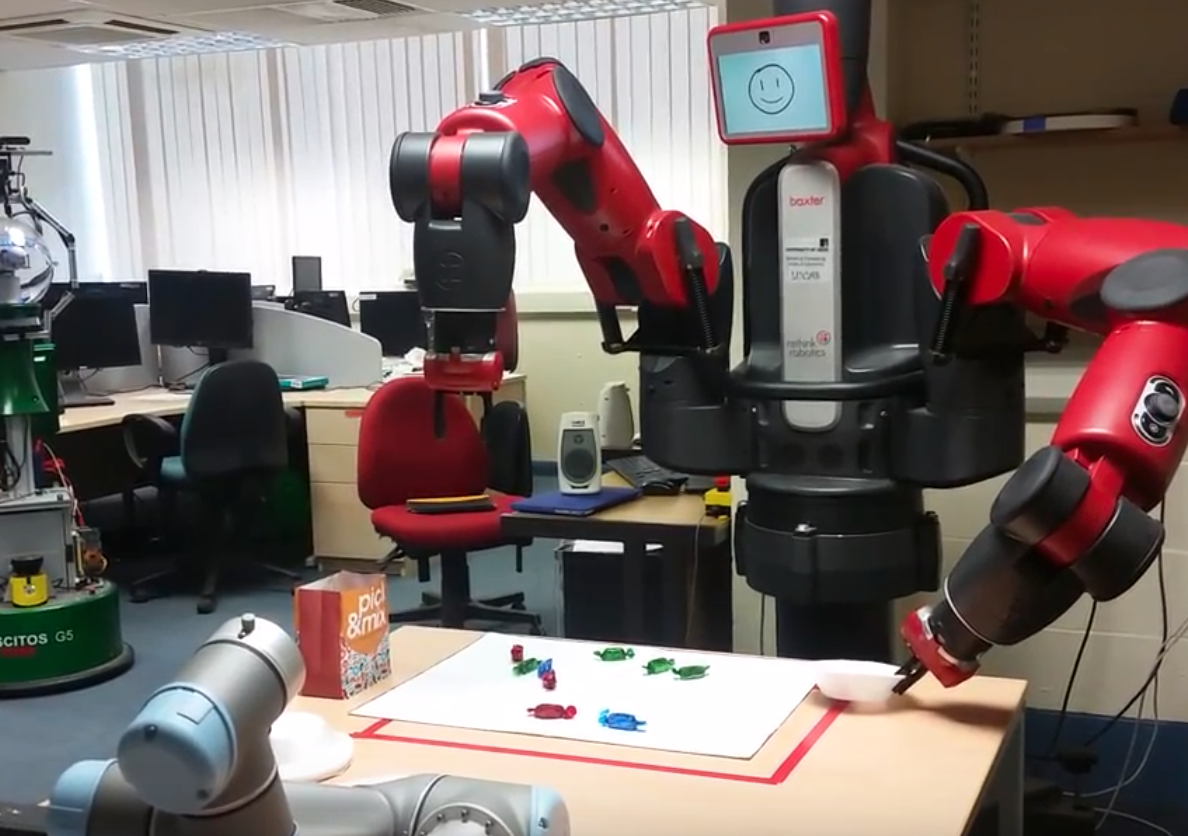
\includegraphics[width=.95\textwidth, height=4.3cm]{8.png}
\end{subfigure}%
}\\
\makebox[\linewidth][c]{%
\begin{subfigure}[b]{.43\textwidth}
\centering
\caption{}
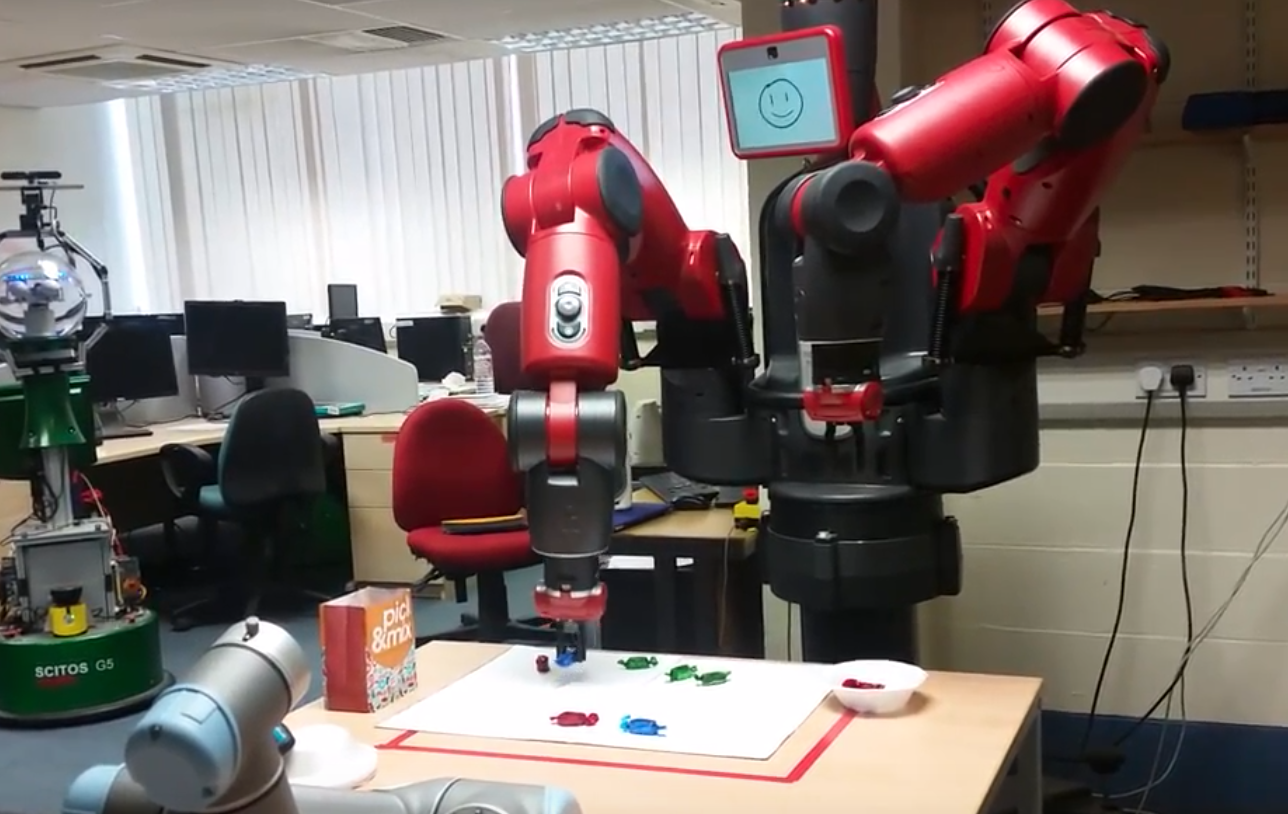
\includegraphics[width=.95\textwidth, height=4.3cm]{11.png}
\end{subfigure}%
\begin{subfigure}[b]{.43\textwidth}
\centering
\caption{}
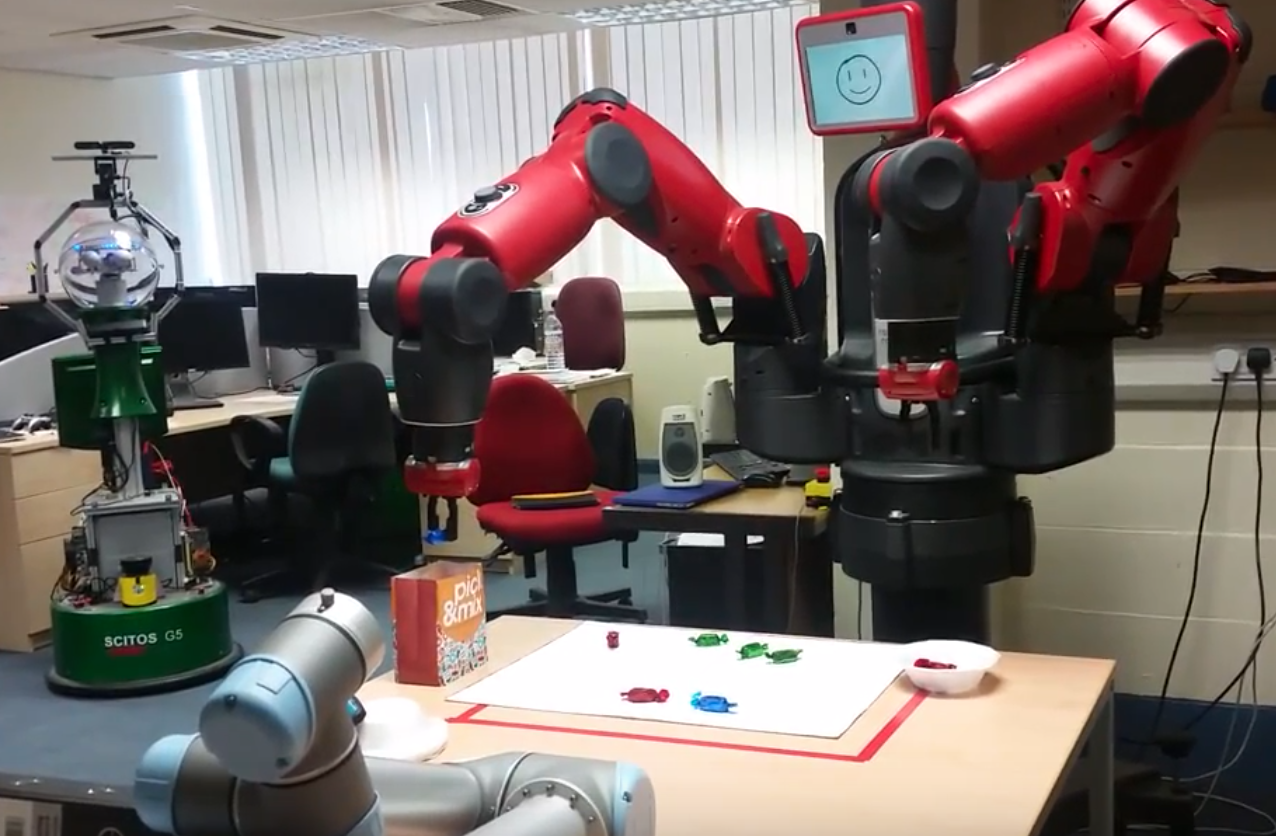
\includegraphics[width=.95\textwidth, height=4.3cm]{12.png}
\end{subfigure}%
\begin{subfigure}[b]{.43\textwidth}
\centering
\caption{}
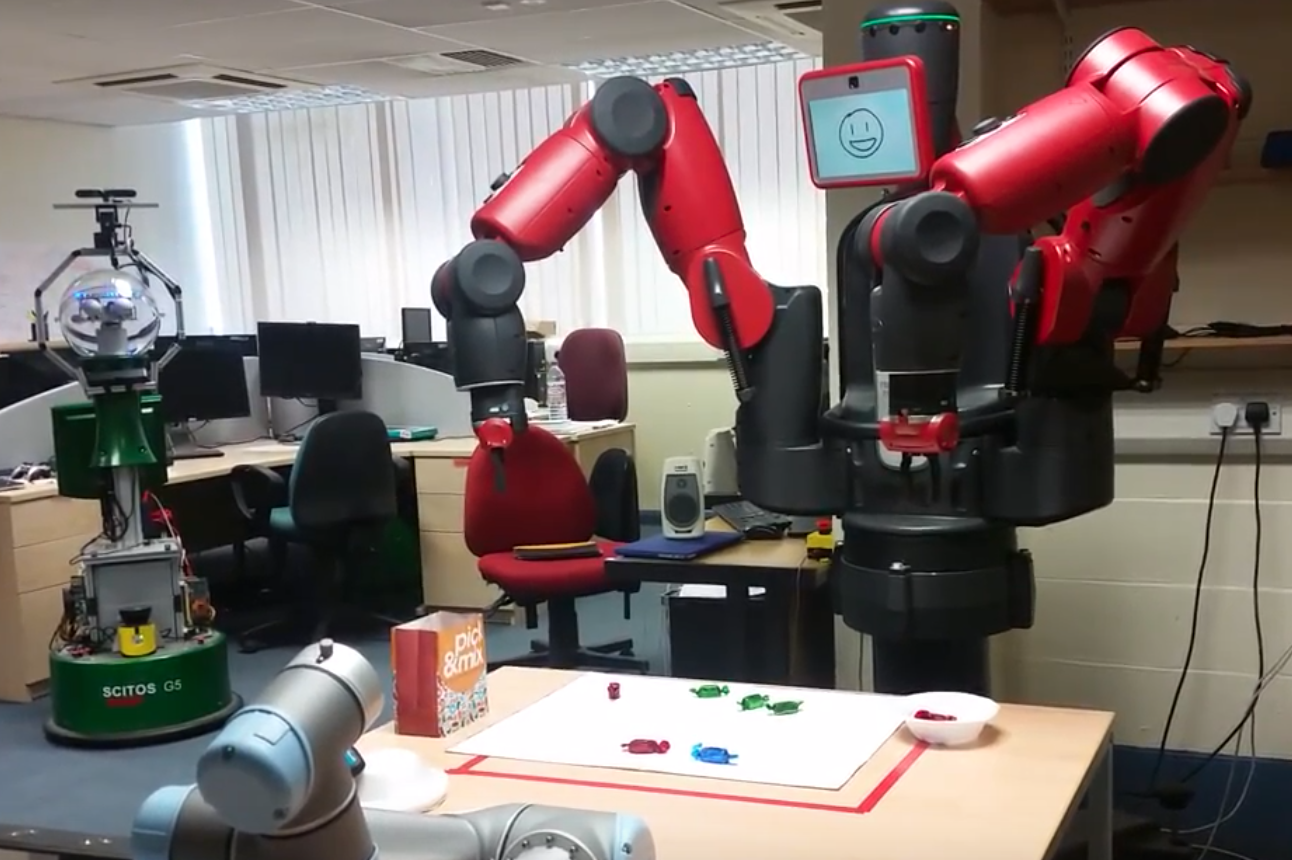
\includegraphics[width=.95\textwidth, height=4.3cm]{13.png}
\end{subfigure}%
}
\caption{An example of the complete working system: (a) Baxter recognises the customer and asks them to provide a voice command for their sweets. (b) The customer says how many blue, red and green sweets they want and confirms on the Android app. (c) Baxter checks the table to make sure there aren't enough sweets on the table already. (d) He looks for the bowl and goes to grab it. (e) The bowl is tipped in two locations above the page. (f) The sweets on the table are scanned, counted and analysed. (g) The requested sweets are grabbed from the table. (h) The grabbed sweets are placed into the sweet bag. (i) Baxter has completed his request, thanks the customer and waits for the next one.}
\label{fig:completeSystem}
\end{figure}
\section{Evaluating the System}
To test the overall system, five different human customers were asked to walk up to Baxter and order some sweets. The reliability of the system was judged on multiple levels: on whether Baxter understood the command, on whether he correctly placed the requested sweets in the bag and on the customer satisfaction with the ease of the process. After doing the human tests, a few observations were made below on the problems encountered.
\newline\newline
Variations in voice/accents provided difficulty for the voice recognition system (although that was expected and more a limitation of the device than the software). Sometimes the voice recognition didn't recognise the colour stated, leaving the rest to be unrecognised too. With more time, multiple accents could be trialled and an increasingly wider search of terms could be accepted for the colours to correct this. Tipping the sweets onto the table, whilst reasonably reliable at separating the sweets, the tilting method still managed to produce hard-to-separate sweet piles. It tended to depend on how the sweets were placed in the bowl initially. As long as the colours and orientations were mixed it seemed OK however, if they were all bunched together in colour order, all facing the same way, a lot of sweets could be tipped out at once. Since the addition of the speech to Baxter, the customers found the interaction reasonably simple to carry out. The face letting the customer know when they were recognised also helped (in case of a slightly inaccurate detection and the customer needed to move about a bit more).
\newline\newline
The trials overall, even after multiple customers had approached Baxter, were very good on the whole, and reliable enough that if Baxter did make a mistake, he knew about it and could correct it. If he missed grabbing a sweet, he would try to grab another, if he hadn't tipped enough sweets on the table to recognise, he would continue tipping until there were enough. Occasionally Baxter grabbed two sweets from a pile instead of one and gave them slightly more than they ordered but that wasn't a important issue. The main issues were on the setup of the system (either the TTS or app server had an issue in starting), but after a reboot of the roslaunch file, the system tended to work well again. 
\section{Limitations/Improvements}
Overall, whilst most of the actions in the shop had been tested to determine reliability, there were still some issues that existed by the end of the project. Here, I will discuss the issues and limitations demonstrated by the final version of the system and approaches I would like to take to these problems if I would have had more time to do so.\newline\newline
\textbf{Human interaction}\newline
The problem with the final interaction system was that there were some gaps in the conversation and interaction that made it not seem lifelike. The main improvements that could have been made with more time were to use a proper skeleton recognition system, so Baxter could constantly recognise the person's skeleton and perform gesture recognition. I feel like the ability for the customer to exchange items with Baxter, such as exchange money or take the bag of sweets would have added to the realism of the interaction greatly. Another issue that was mentioned was to implement threading and idle movements. Threading would have helped Baxter move both arms together in more human-like movements (instead of moving them one at a time). Idle movements were discussed as an addition to make Baxter seem lifelike even when he was not talking to a customer. As future tasks, it would be nice for those to be implemented so at the open day, Baxter would not be stood still until a customer approached him.
\newline\newline
\textbf{Sweet Recognition}\newline
Whilst this system was reasonably reliable by the end (and a lot more efficient than it was in initial iterations), there were still some problems that needed to be rectified. To be more robust, the sweet recognition system should have been made to work within different shop-like settings. The problem was different light sources would affect the testing data used to train the neural network. Therefore if the shop had a different coloured light source, the sweet colour recognition would be unreliable. I think a good way to solve this problem would be to add a user setup method to train new sweets under new conditions and automate the process. That would mean a user could then run the software, place multiple target sweets onto the table and Baxter would record their data and train the neural network. That addition to the system would certainly make it easier and more robust to be used in different rooms throughout the university for open days.\newline\newline
\textbf{Sweet Singulation}\newline
If there was more time, a more efficient sweet singulation algorithm would be proposed/developed. The problem with singulating the sweets vision-wise and manipulation-wise is that there was no clear way to do this task. I carried out a lot of research and there is no specified way to be able to recognise individual, deformable objects within a cluster, with variable shape and colour. The fact that the sweets could vary in shape so much, meant that most vision techniques using shape recognition would not work - for example, template matching was considered but it could not be reliably implemented. The variation in colour meant that the sweets could not be differentiated easily by colour as all three wrapper colours could overlap in the HSV or RGB colourspace. Therefore, the combined method I used, using colour detection, then other processing methods was the best method I could manage to implement, but with more time, I think there would be a more accurate, computationally efficient approach to solve this.
\section{Project Reflection}
Over the past twelve weeks, I have really enjoyed this project and I think that mainly, it went very well and I am pleased with the overall deliverables produced. The main problem I think I had was organisation of time. After doing the initial planning report and the supervisor/assessor presentation at week 8, the main issues with the feedback from both those meetings were that the time limit was overly ambitious and at some point, some features would have to be cut out. By the end of the project, there were multiple discussed parts of the project that were not developed: money exchange with the customer and fully developed sweet singulation were some of the key features that I didn't have time to complete. Whilst money exchange with the customer was a stretch goal anyway, the sweet singulation methods turned out to be a lot more of a complex issue than initially proposed.
\newline\newline
If I were to do the project again, I think I would have started coding and work on the project earlier. A major issue was that I started developing the bowl recognition system with the Kinect as the first task. It took a long time to get used to the methods and PCL libraries. The problem was that the first main coding task was based on two completely new pieces of software: ROS and the PCL library. I feel that if I had started with the simpler OpenCV/Python based coding tasks first, it would've made the project easier to start and develop and could have prevented getting stuck for as long in the initial few weeks. Possibly the reason why the bowl recognition task took so long is because ROS was quite difficult to pick up and use and there wasn't a lot of great documentation out there to explain the core concepts of it. Once I got to around week 6, I felt like I fully understood the principles of ROS and could therefore do a lot more with it.
\newline\newline
Looking back at the initial objectives, they stated I needed to develop a vision system for the bowl, sweets, a manipulation system for them and a some human interaction systems. I believe that I have achieved all of these basic objectives to some extent and am very happy with the quality of the results produced at each stage. I thoroughly enjoyed the overall project and feel like I got a lot out of it. The weekly meetings with my supervisor were very useful, to discuss and develop ideas with but mainly, I feel a sense of achievement that I mainly developed this entire project on my own.

%Adds References to the table of content
%all you bibtex enteries go in the file called refs.bib
\addcontentsline{toc}{chapter}{References}
\bibliographystyle{unsrt}
\bibliography{refs}

%any appendices you have go in a file called appendix.
\begin{appendices}
\let\cleardoublepage\clearpage
\chapter{External Materials}
In this project, there were many external materials used for inspiration and development. For this reason, any ROS nodes that are publically available, were not included in this section as the ones used are already mentioned in the report.
\newline\newline
Within the project files:\newline\newline
One of the PhD students within the robotics lab has a github: \url{https://github.com/OMARI1988}. His code provided a lot of the inspiration for mine so parts were taken from his publically hosted projects: \textbf{objectfinder.py} was directly taken from the github, as was some of the setup code for Baxter's movement, adapted from the robotics tabletop/board game code.\newline\newline
Other code used externally tended to be from documentation and tutorials, which are referenced in footnotes throughout the project where necessary.
\chapter{Ethical Issues Addressed}
Whilst in this project, there weren't many ethical issues to address, one has to consider the implications of AI in general with this type of task. In the customer-shopkeeper interaction, Baxter `observes' customers and passers-by throughout the running of the software. In the robotics department, I came across other PhD students having difficulty gaining consent for taking Kinect recordings of skeletons. Whilst Baxter doesn't expressly record them, it could stray into the grey area of whether the person should give their permission to have their images taken/analysed by Baxter in the first place.
\end{appendices}
\end{document}

